%-----------------------Homework------------------------------------
%-------------------Arman Shokrollahi---------------------------------
%---------------------Coding Theory-------------------------------

\documentclass[a4 paper]{article}
% Set target color model to RGB
\usepackage[inner=1.5cm,outer=1.5cm,top=2.5cm,bottom=2.5cm]{geometry}
\usepackage{setspace}
\usepackage[rgb]{xcolor}
\usepackage{pythonhighlight}
\usepackage{caption}
\usepackage{subcaption}
\usepackage{pdfpages}
\usepackage{verbatim}
\usepackage{amsgen,amsmath,amstext,amsbsy,amsopn,tikz,amssymb,tkz-linknodes}
\usepackage{fancyhdr}
\usepackage[colorlinks=true, urlcolor=blue,  linkcolor=blue, citecolor=blue]{hyperref}
\usepackage[colorinlistoftodos]{todonotes}
\usepackage{rotating}
%\usetikzlibrary{through,backgrounds}
\hypersetup{%
pdfauthor={Arman Shokrollahi},%
pdftitle={Homework},%
pdfkeywords={Tikz,latex,bootstrap,uncertaintes},%
pdfcreator={PDFLaTeX},%
pdfproducer={PDFLaTeX},%
}
%\usetikzlibrary{shadows}
\usepackage[francais]{babel}
\usepackage{booktabs}
\newcommand{\ra}[1]{\renewcommand{\arraystretch}{#1}}

      \newtheorem{thm}{Theorem}[section]
      \newtheorem{prop}[thm]{Proposition}
      \newtheorem{lem}[thm]{Lemma}
      \newtheorem{cor}[thm]{Corollary}
      \newtheorem{defn}[thm]{Definition}
      \newtheorem{rem}[thm]{Remark}
      \numberwithin{equation}{section}

\newcommand{\homework}[6]{
   \pagestyle{myheadings}
   \thispagestyle{plain}
   \newpage
   \setcounter{page}{1}
   \noindent
   \begin{center}
   \framebox{
      \vbox{\vspace{2mm}
    \hbox to 6.28in { {\bf JWST Project \hfill} }
       \vspace{6mm}
       \hbox to 6.28in { {\Large \hfill #1 (#2)  \hfill} }
       \vspace{6mm}
       \hbox to 6.28in { {\it Instructor: #3 \hfill Student: #5} }
       %\hbox to 6.28in { {\it TA: #4  \hfill #6}}
      \vspace{2mm}}
   }
   \end{center}
   \markboth{#5 -- #1}{#5 -- #1}
   \vspace*{4mm}
}

\newcommand{\bbF}{\mathbb{F}}
\newcommand{\bbX}{\mathbb{X}}
\newcommand{\bI}{\mathbf{I}}
\newcommand{\bX}{\mathbf{X}}
\newcommand{\bY}{\mathbf{Y}}
\newcommand{\bepsilon}{\boldsymbol{\epsilon}}
\newcommand{\balpha}{\boldsymbol{\alpha}}
\newcommand{\bbeta}{\boldsymbol{\beta}}
\newcommand{\0}{\mathbf{0}}

\begin{document}
\homework{Meeting Notes \#4}{due 03/15/23 }{McCleary}{}{Eddie Berman}{}
{\begin{tikzpicture}[outline/.style={draw=#1,thick,fill=#1!50}]
\node [outline=red] at (0,1) {\bf Agenda};
\end{tikzpicture}}
\begin{enumerate}
    \item New results from PSF
    \item Applications Done (+ optimism)
    \item SUMS Saturday
    \item Been reading \href{https://press.princeton.edu/absil}{Absil}
\end{enumerate}

\noindent {\fbox{\it PSF Results}}\\ 
\section{30mas Control}
\begin{python}
# How large should the postage stamp cutouts of the stars be?
    stamp_size: 30

model:
    # This model uses a grid of pixels to model the surface brightness distribution.
    type: PixelGrid
    scale: 0.025      # NIRCam ative pixel scale
    size: 26          # Model is 24 x 24 in these pixels
\end{python}
\begin{figure}[!h]
  \begin{subfigure}{\linewidth}
  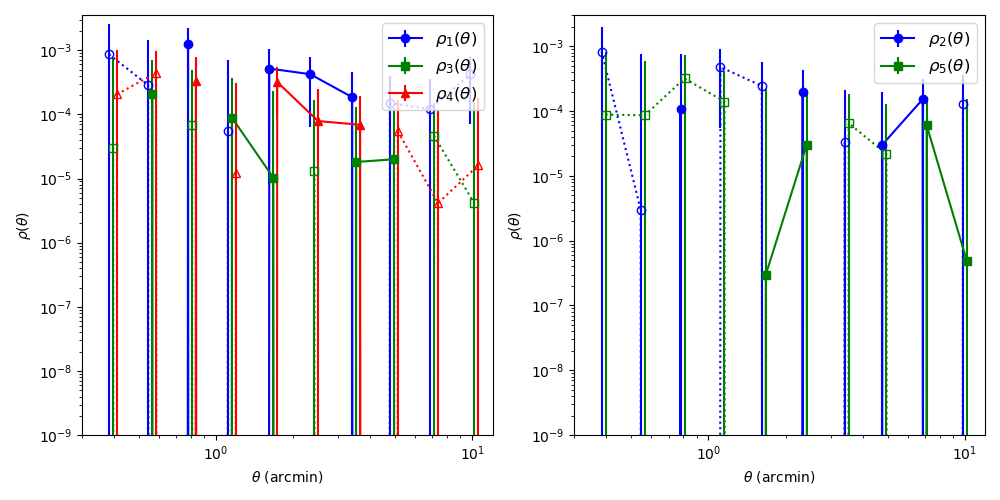
\includegraphics[width=.3\linewidth]{30Control/piff_rho.png}\hfill
  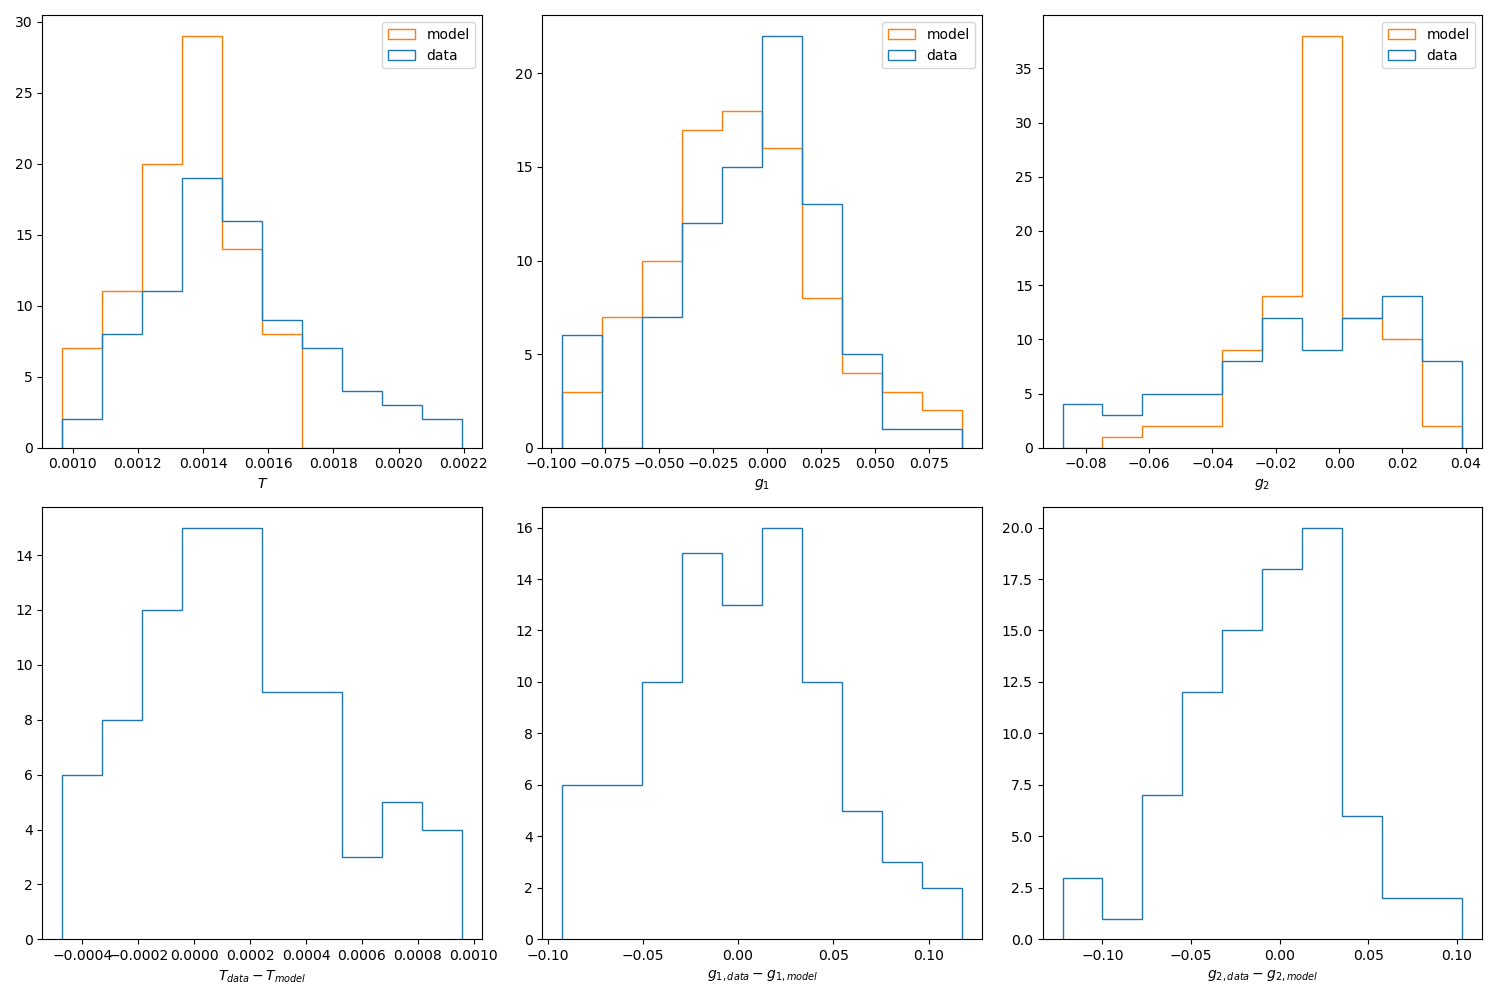
\includegraphics[width=.3\linewidth]{30Control/piff_shapes.png}\hfill
  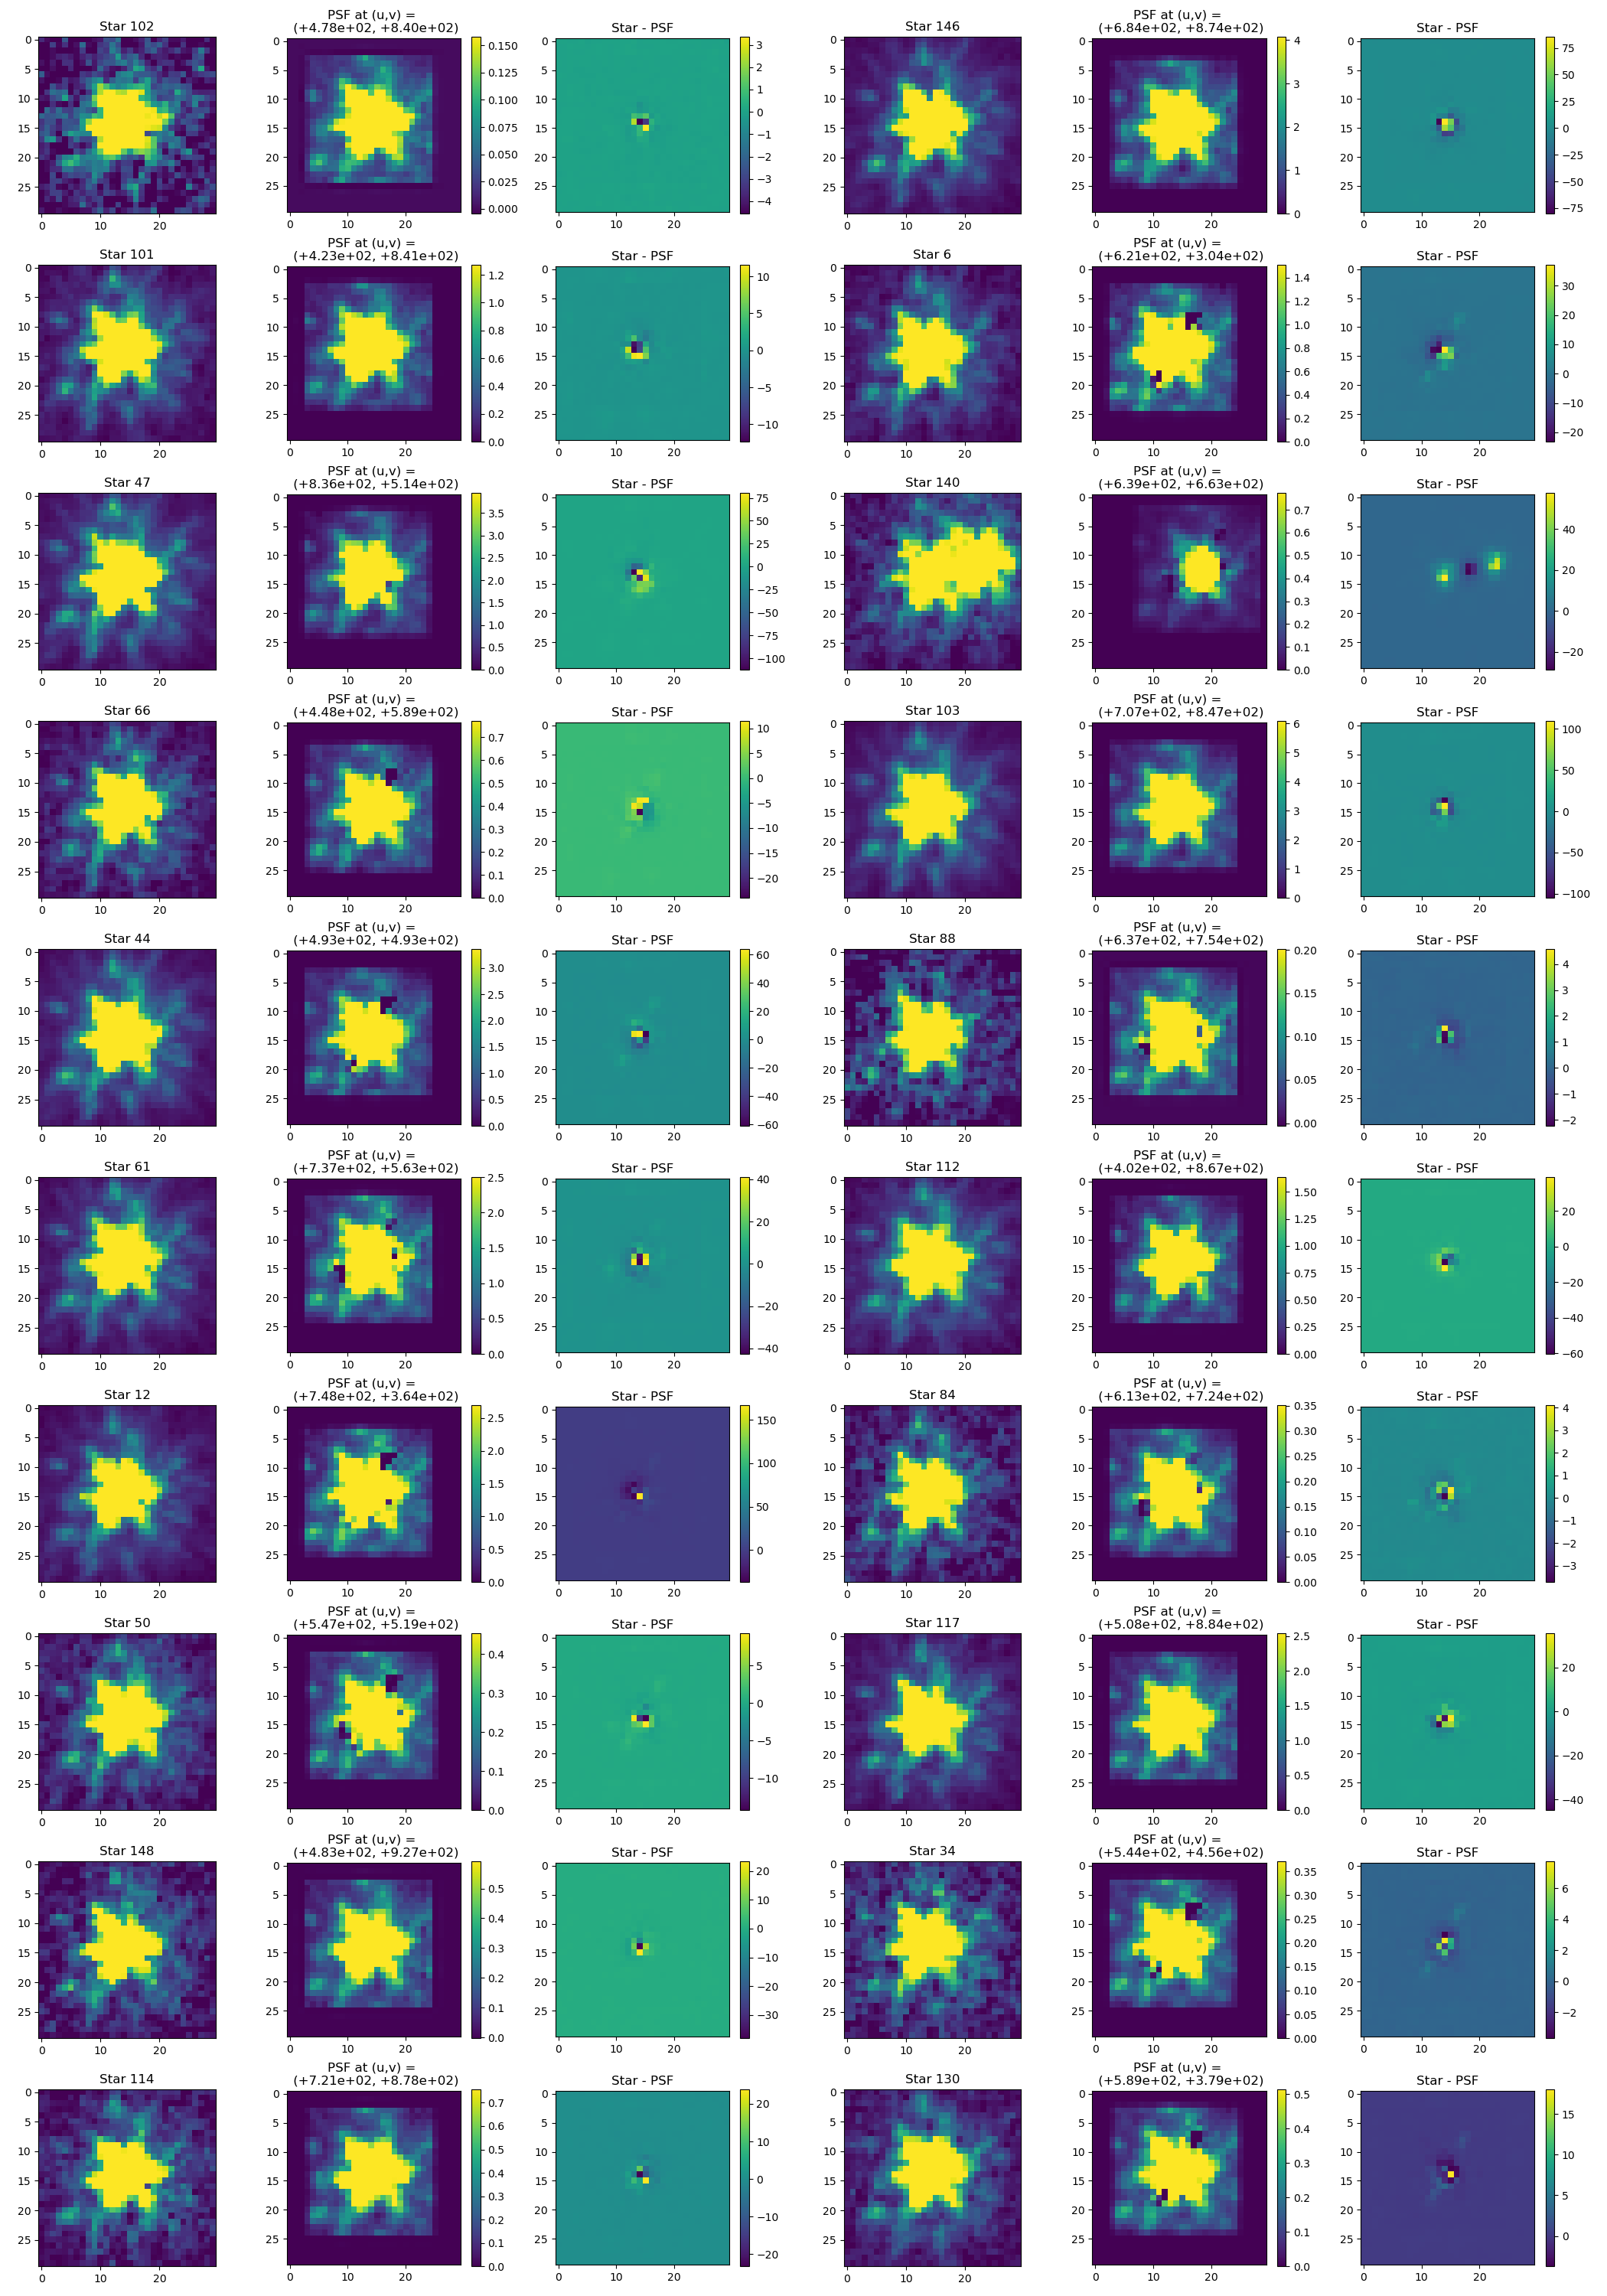
\includegraphics[width=.3\linewidth]{30Control/piff_stars.png}
  \end{subfigure}\par\medskip
  \begin{subfigure}{\linewidth}
  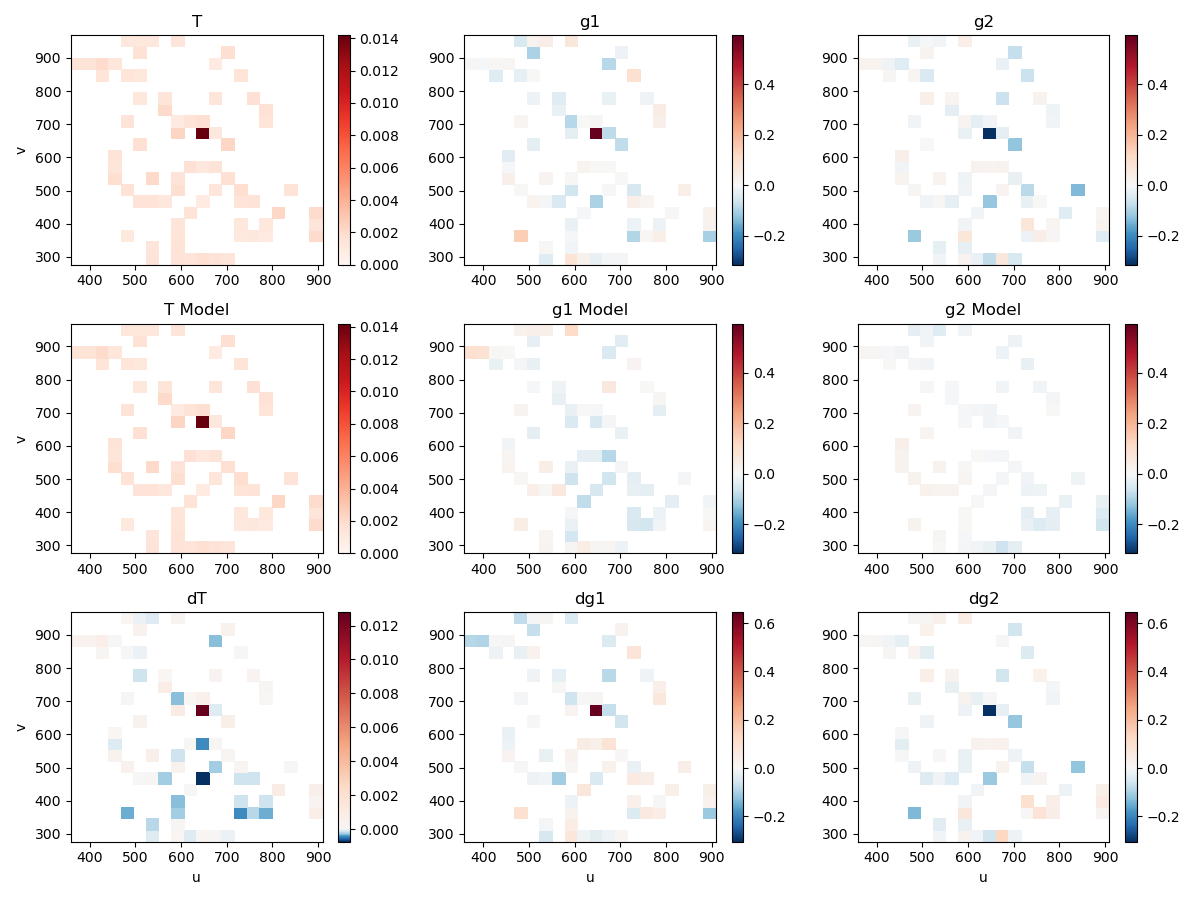
\includegraphics[width=.3\linewidth]{30Control/piff_twod.png}\hfill
  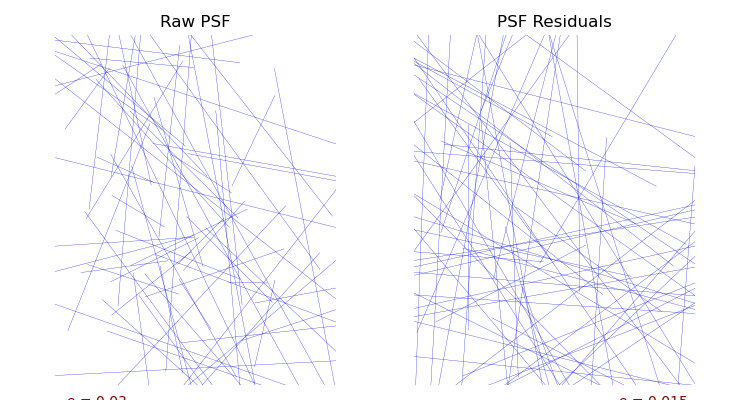
\includegraphics[width=.3\linewidth]{30Control/piff_whisker.png}\hfill
  \caption{f115w 30mas Control}
  \end{subfigure}\par\medskip


\end{figure} \clearpage
\section{30mas Experimental}
\begin{python}
# How large should the postage stamp cutouts of the stars be?
    stamp_size: 30

model:
    # This model uses a grid of pixels to model the surface brightness distribution.
    type: PixelGrid
    scale: 0.0175      # NIRCam ative pixel scale
    size: 40          # Model is 24 x 24 in these pixels
\end{python}
\begin{figure}[!h]
  \begin{subfigure}{\linewidth}
  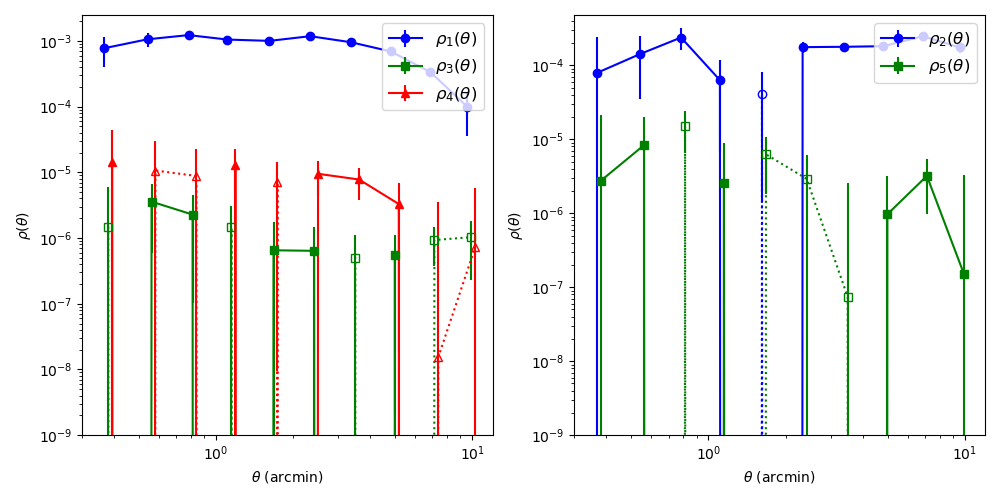
\includegraphics[width=.3\linewidth]{150/piff_rho.png}\hfill
  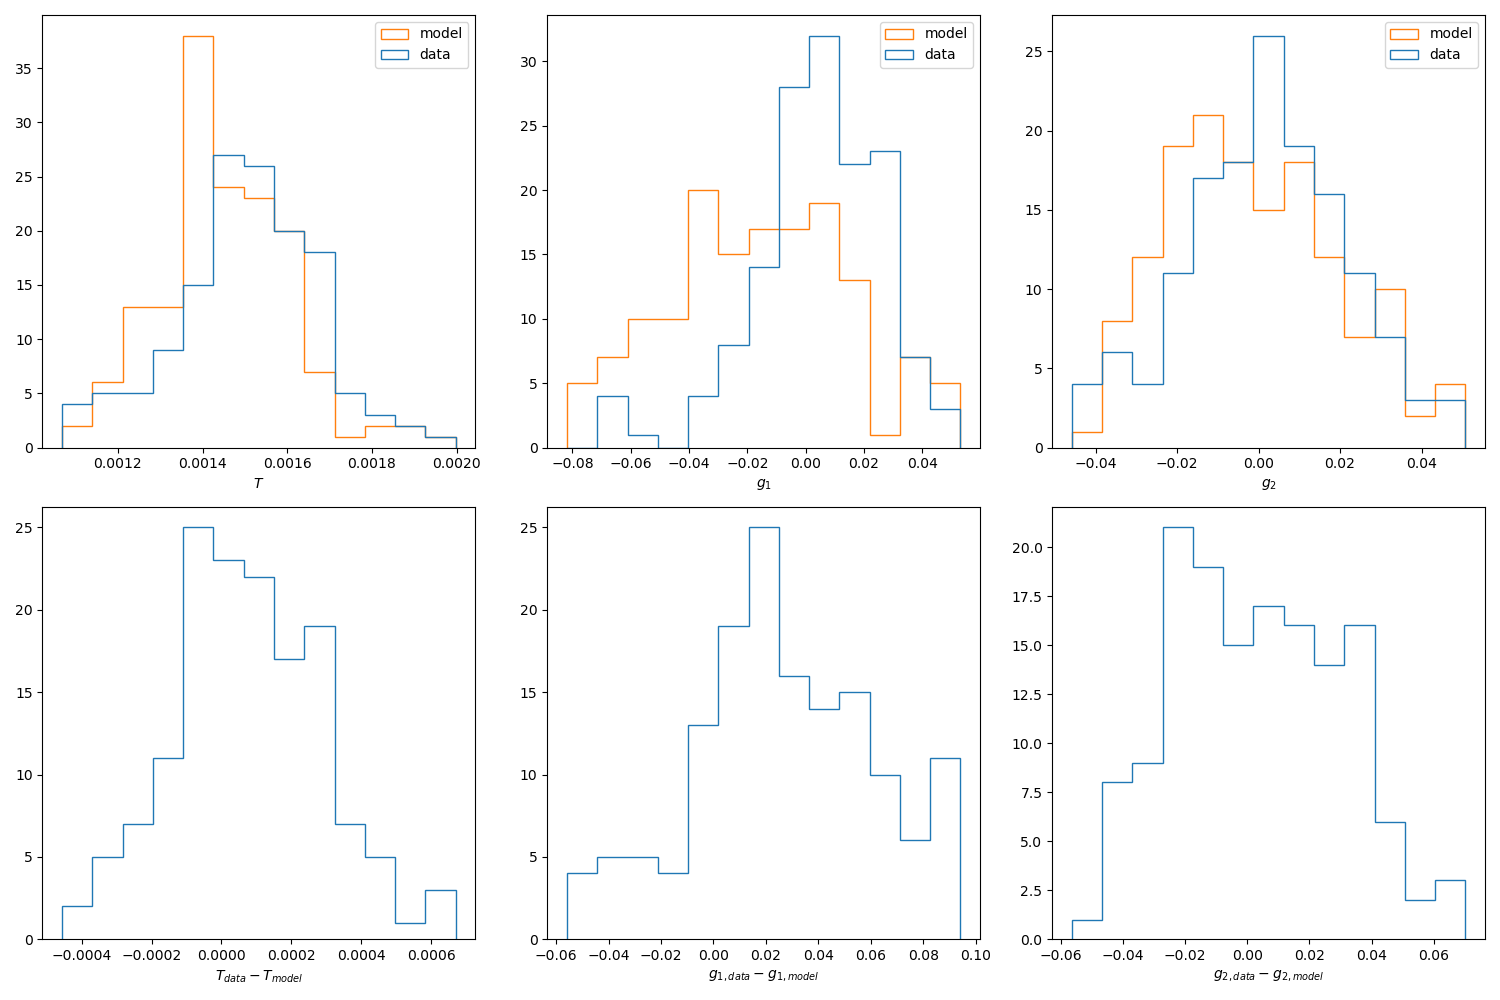
\includegraphics[width=.3\linewidth]{150/piff_shapes.png}\hfill
  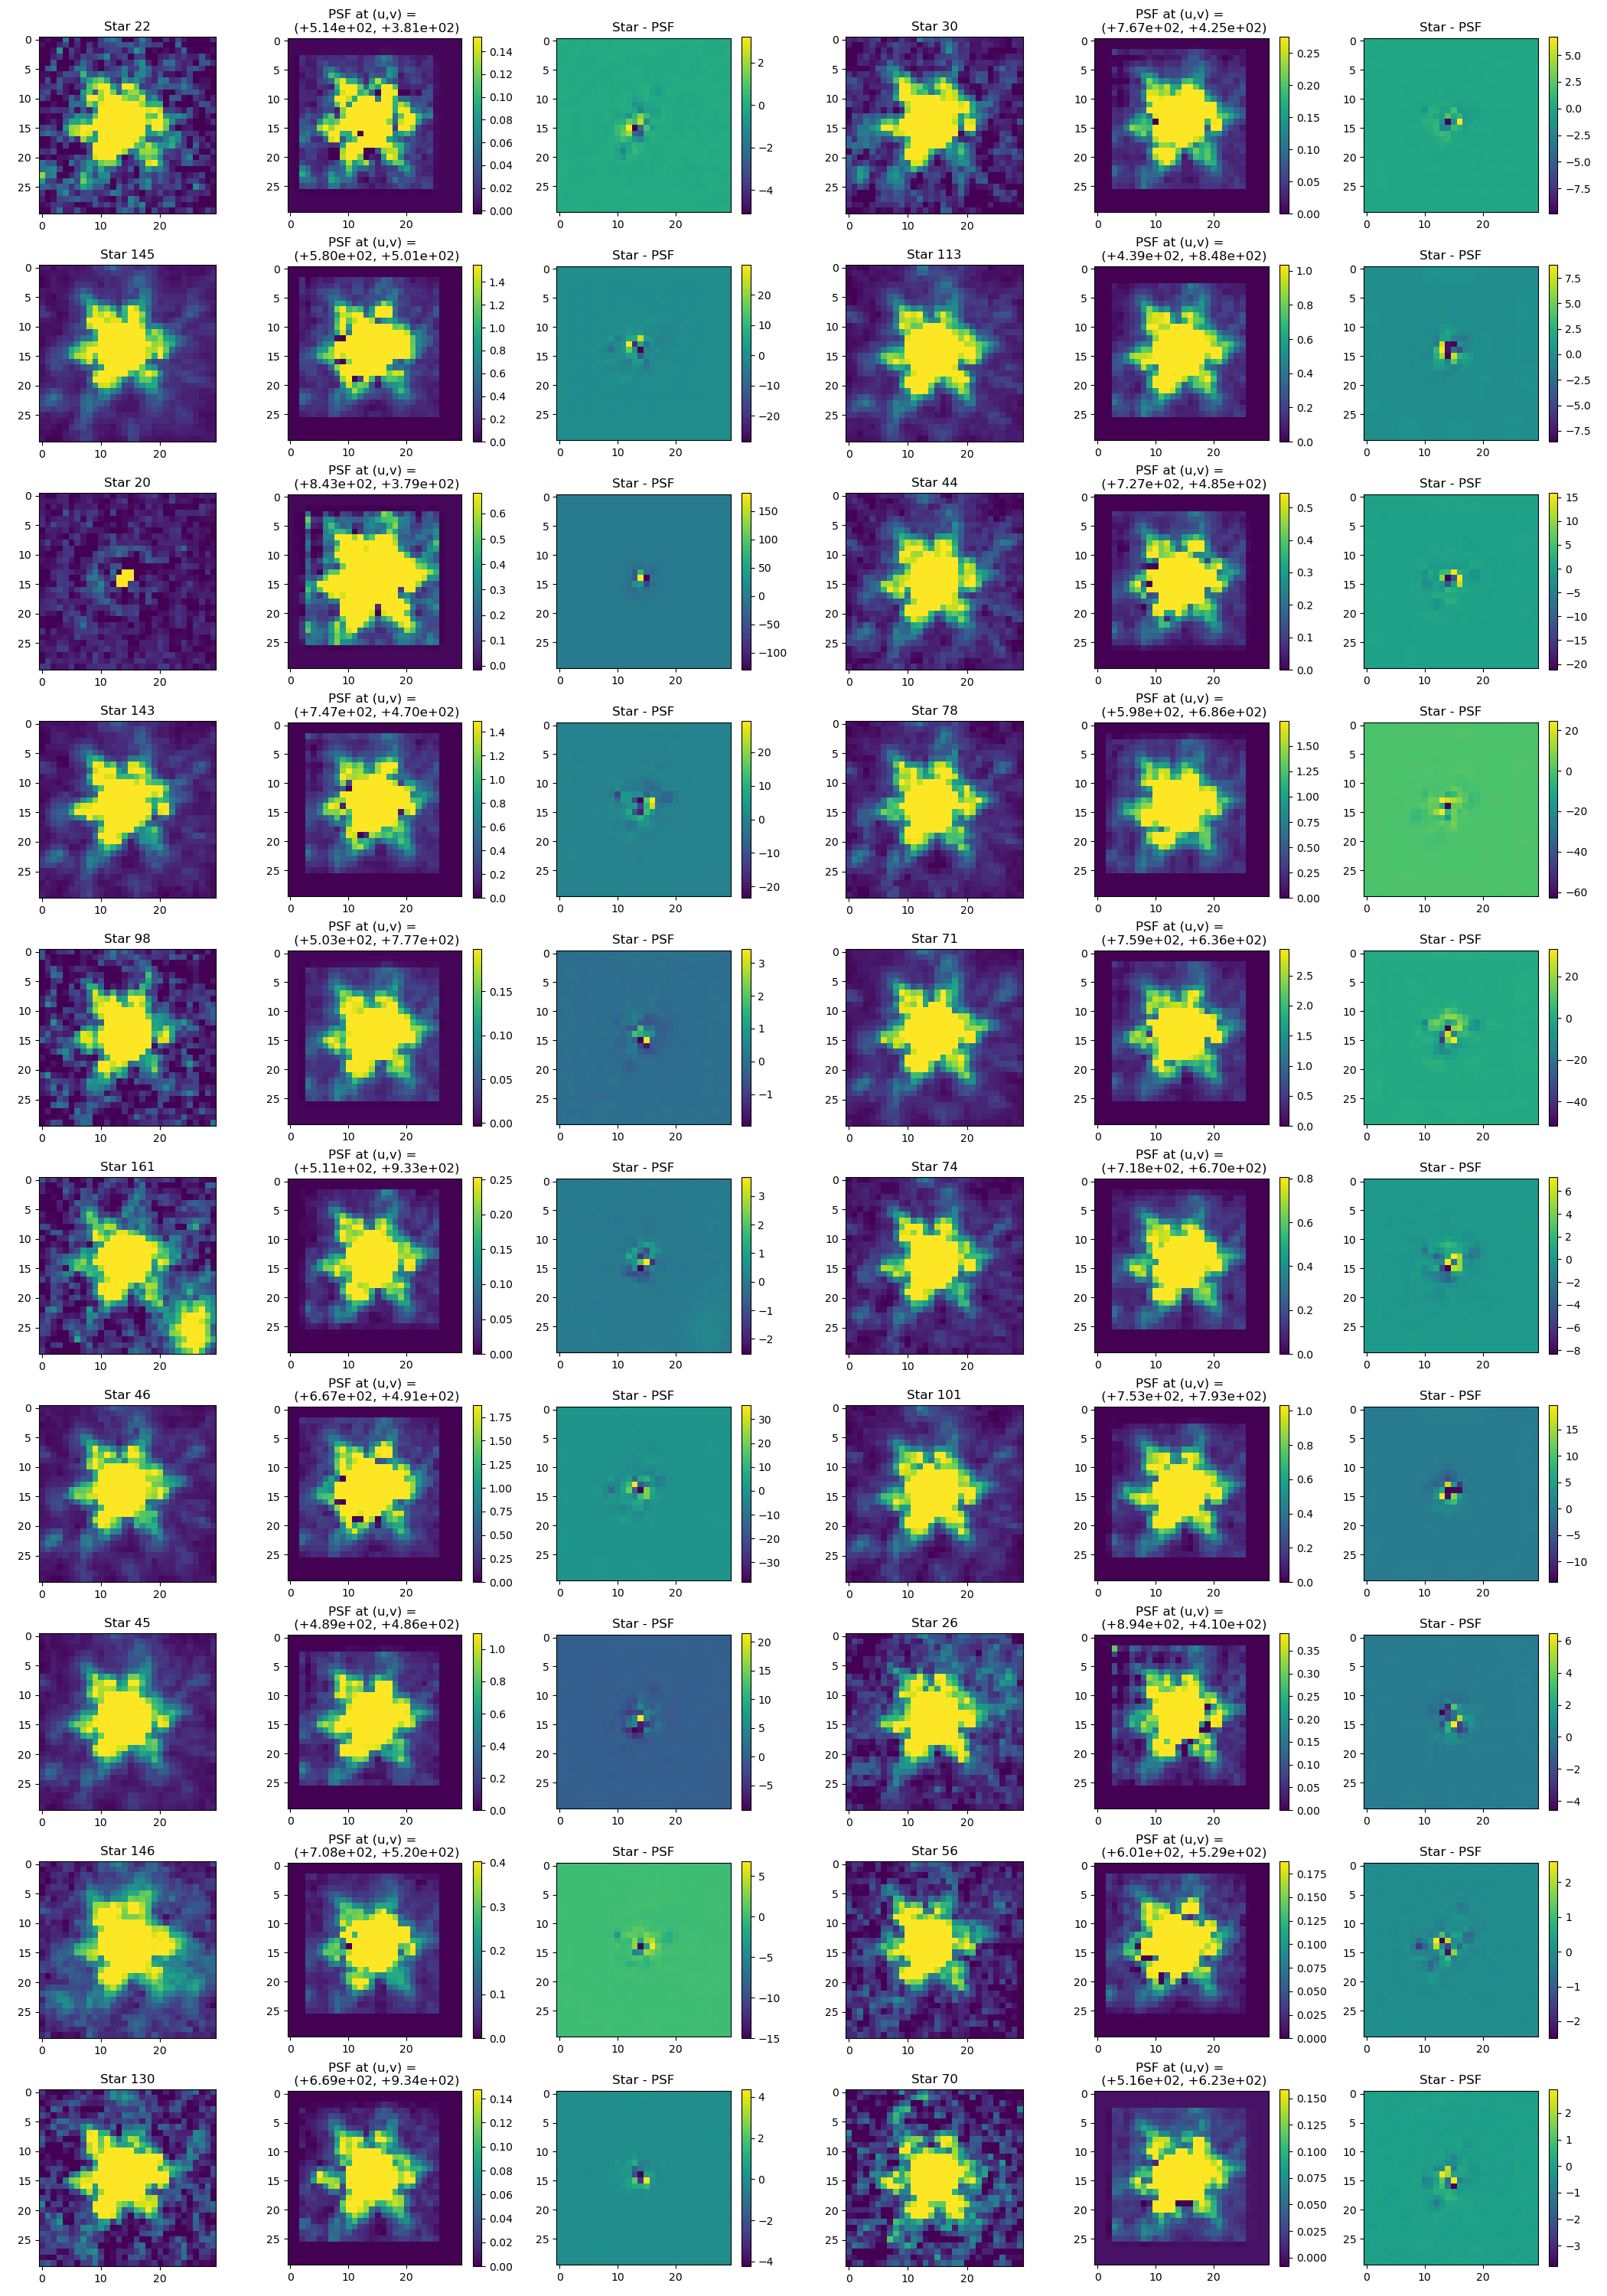
\includegraphics[width=.3\linewidth]{150/piff_stars.png}
  \end{subfigure}\par\medskip
  \begin{subfigure}{\linewidth}
  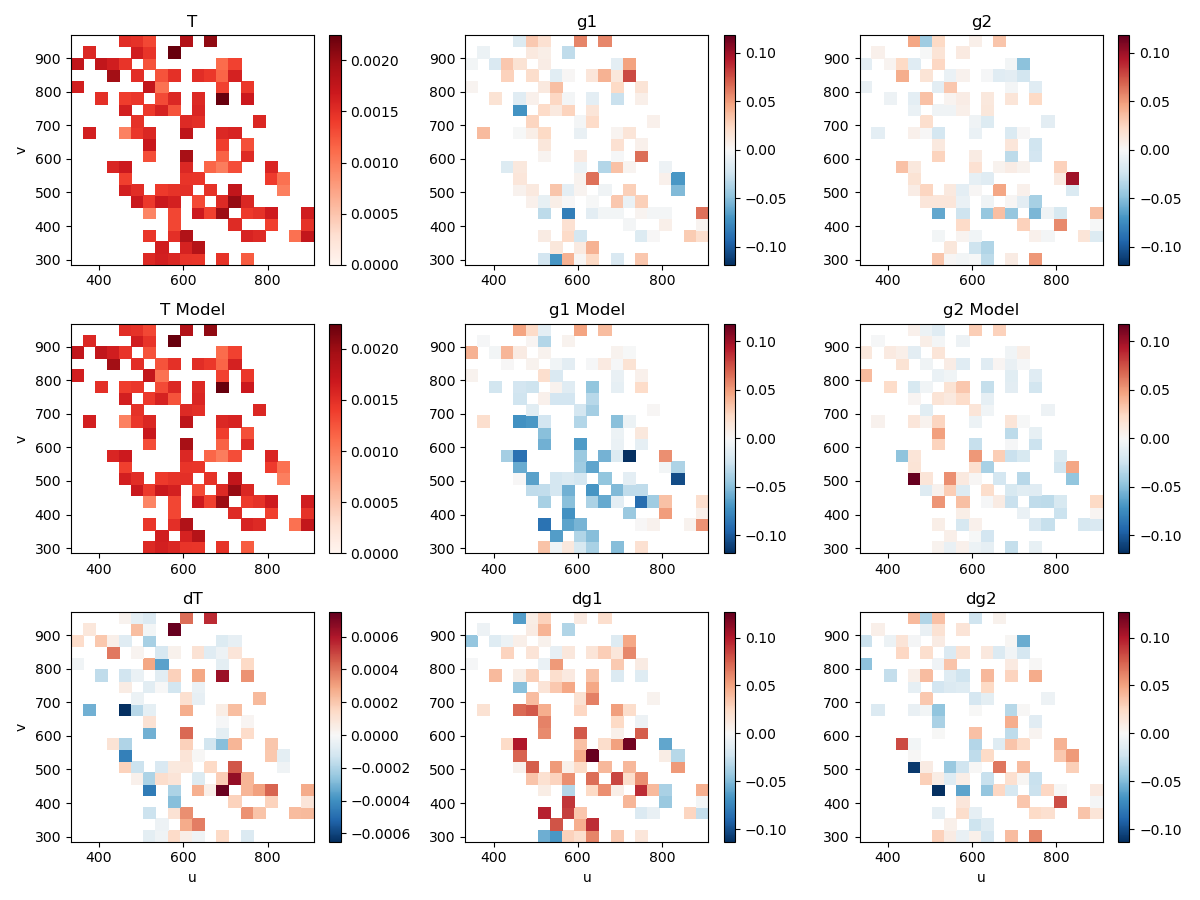
\includegraphics[width=.3\linewidth]{150/piff_twod.png}\hfill
  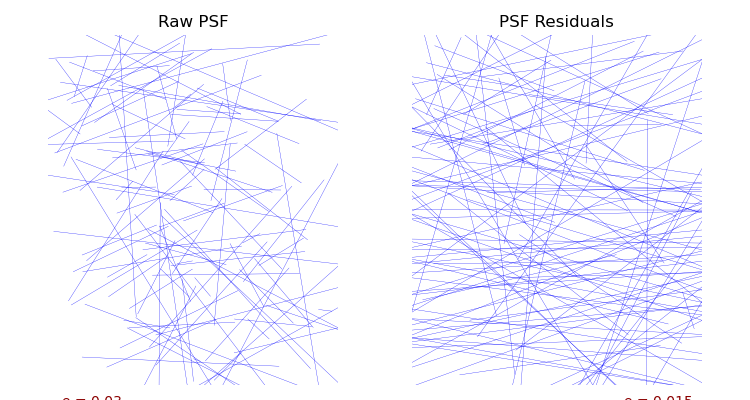
\includegraphics[width=.3\linewidth]{150/piff_whisker.png}\hfill
  \caption{f150w 30mas experimental}
  \end{subfigure}\par\medskip


\end{figure}
\begin{figure}[!h]
  \begin{subfigure}{\linewidth}
  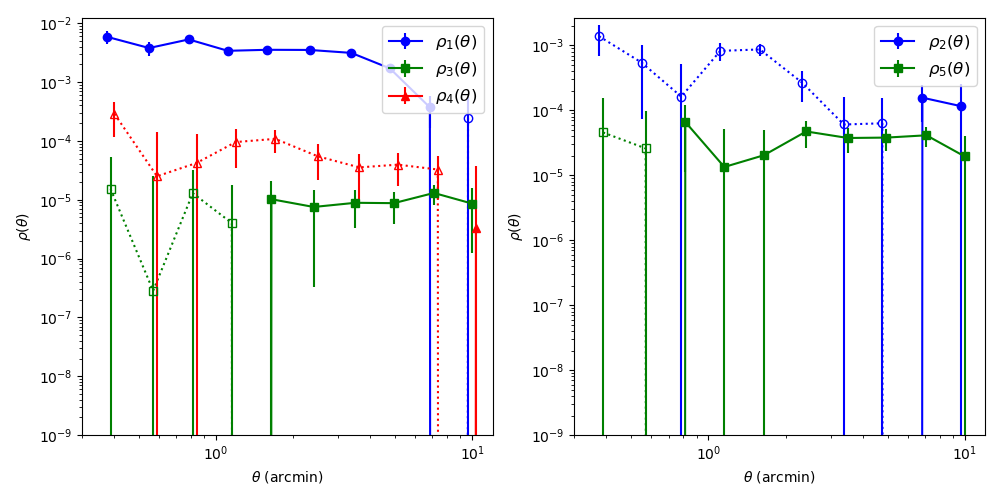
\includegraphics[width=.3\linewidth]{115_30/piff_rho.png}\hfill
  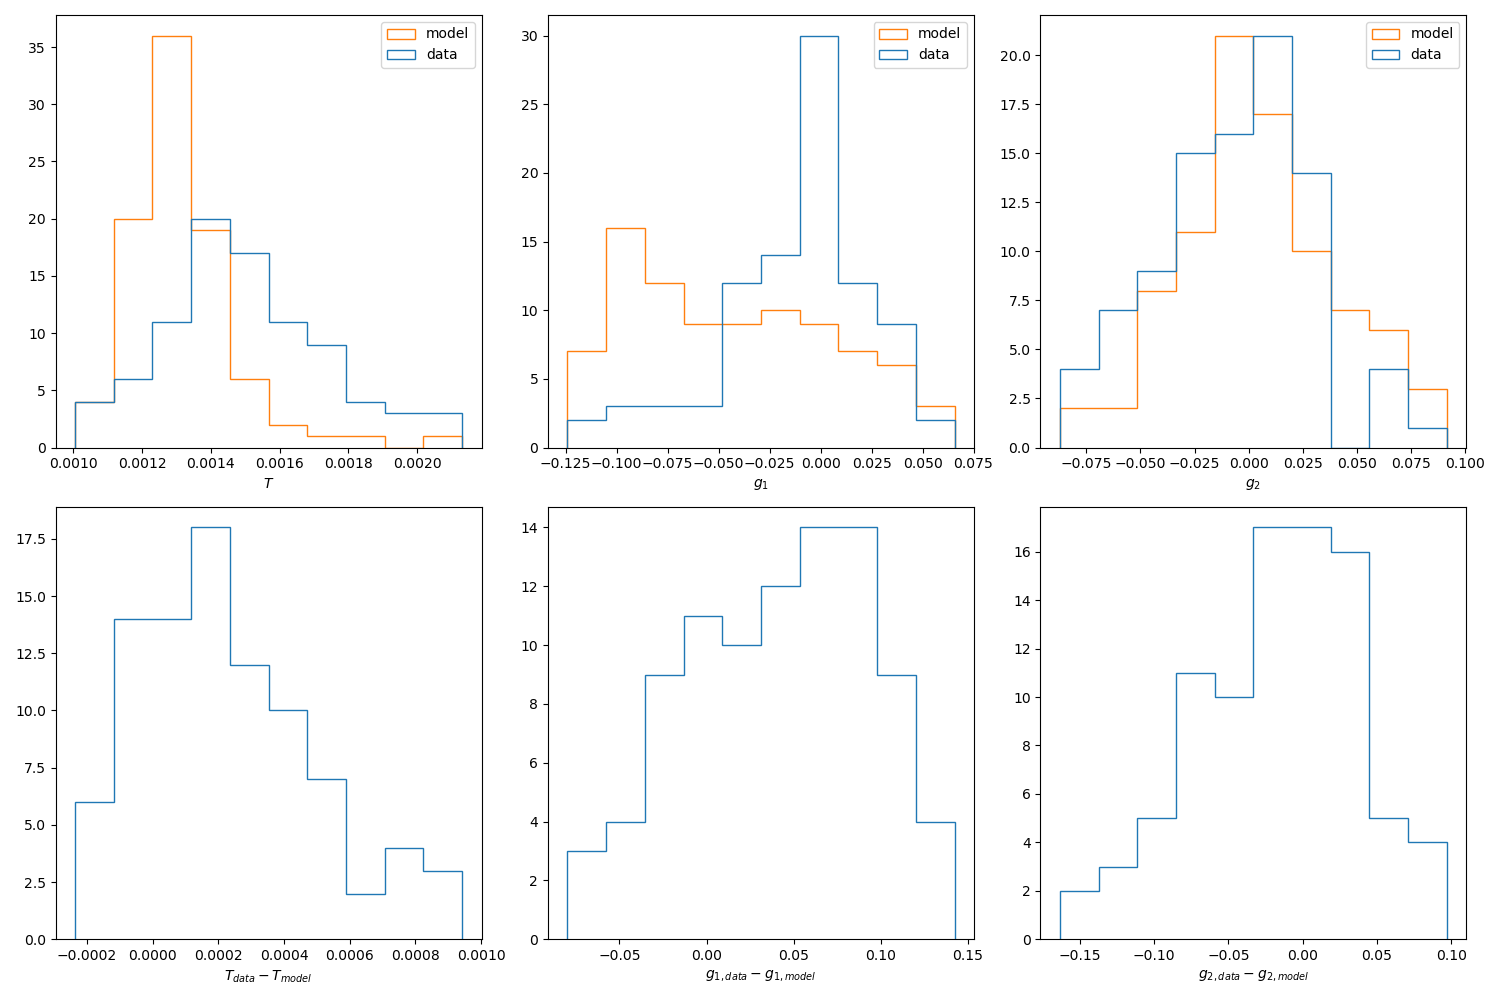
\includegraphics[width=.3\linewidth]{115_30/piff_shapes.png}\hfill
  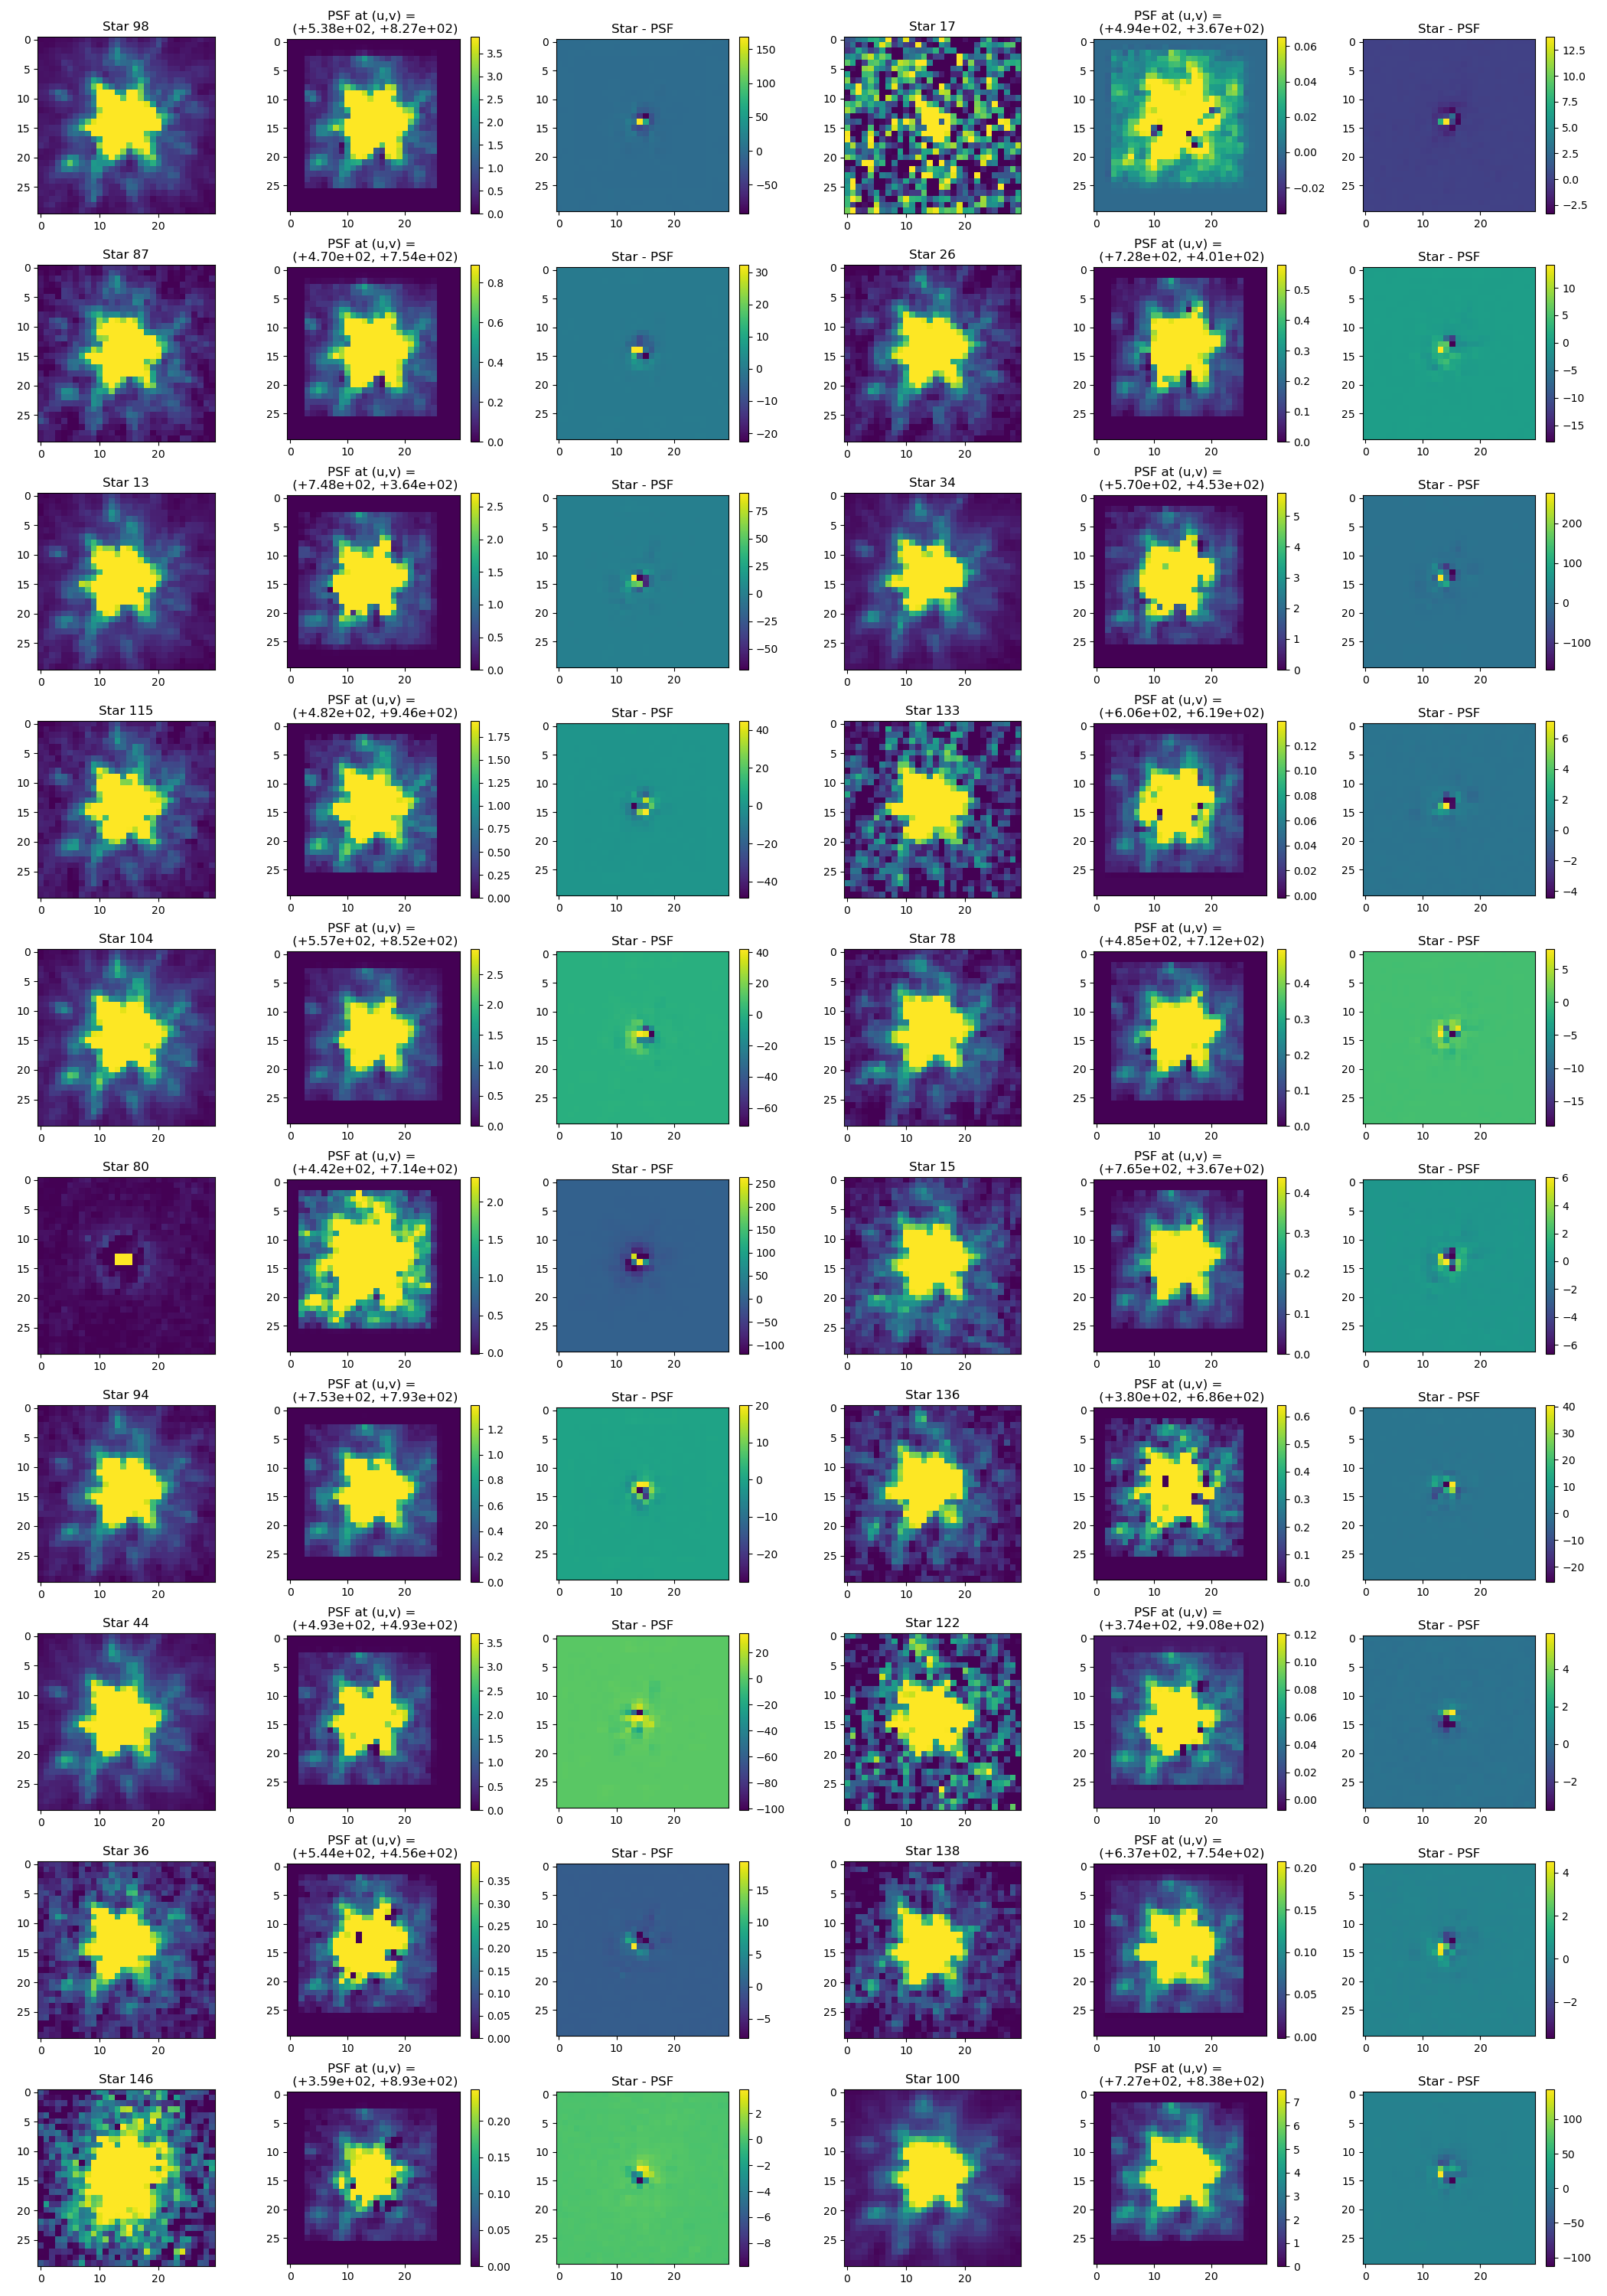
\includegraphics[width=.3\linewidth]{115_30/piff_stars.png}
  \end{subfigure}\par\medskip
  \begin{subfigure}{\linewidth}
  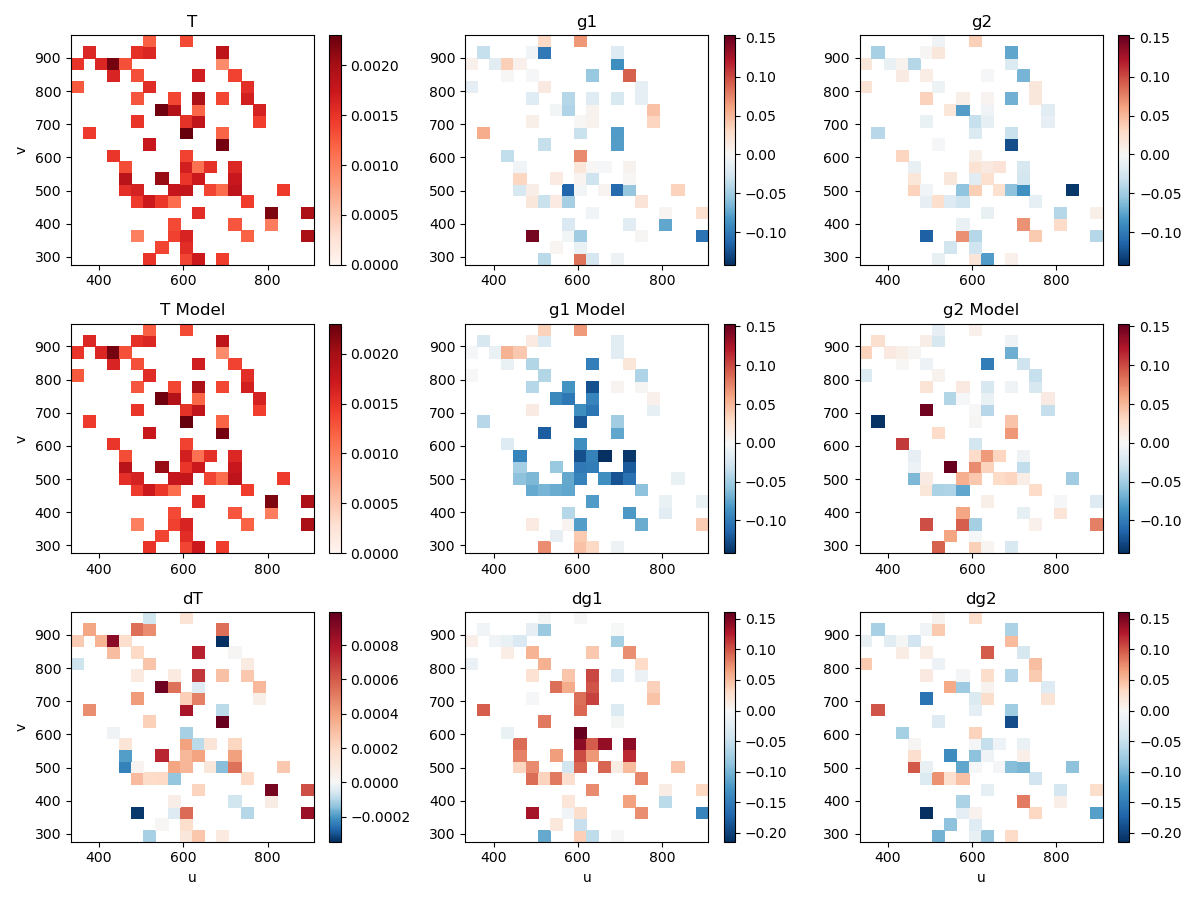
\includegraphics[width=.3\linewidth]{115_30/piff_twod.png}\hfill
  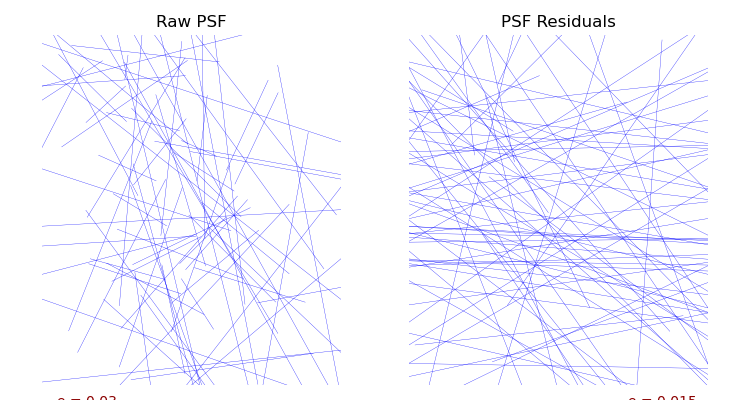
\includegraphics[width=.3\linewidth]{115_30/piff_whisker.png}\hfill
  \caption{f150w 30mas}
  \end{subfigure}\par\medskip


\end{figure}
\begin{figure}[!h]
  \begin{subfigure}{\linewidth}
  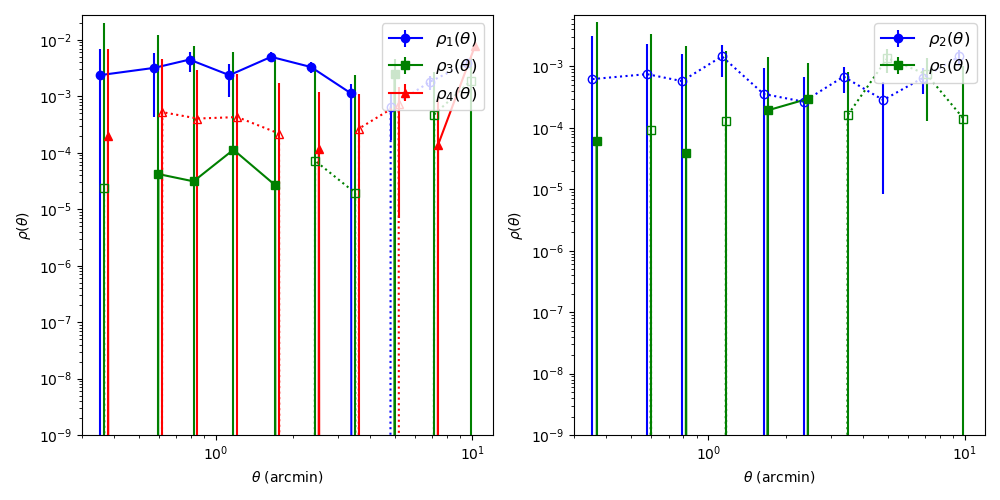
\includegraphics[width=.3\linewidth]{277.30/piff_rho.png}\hfill
  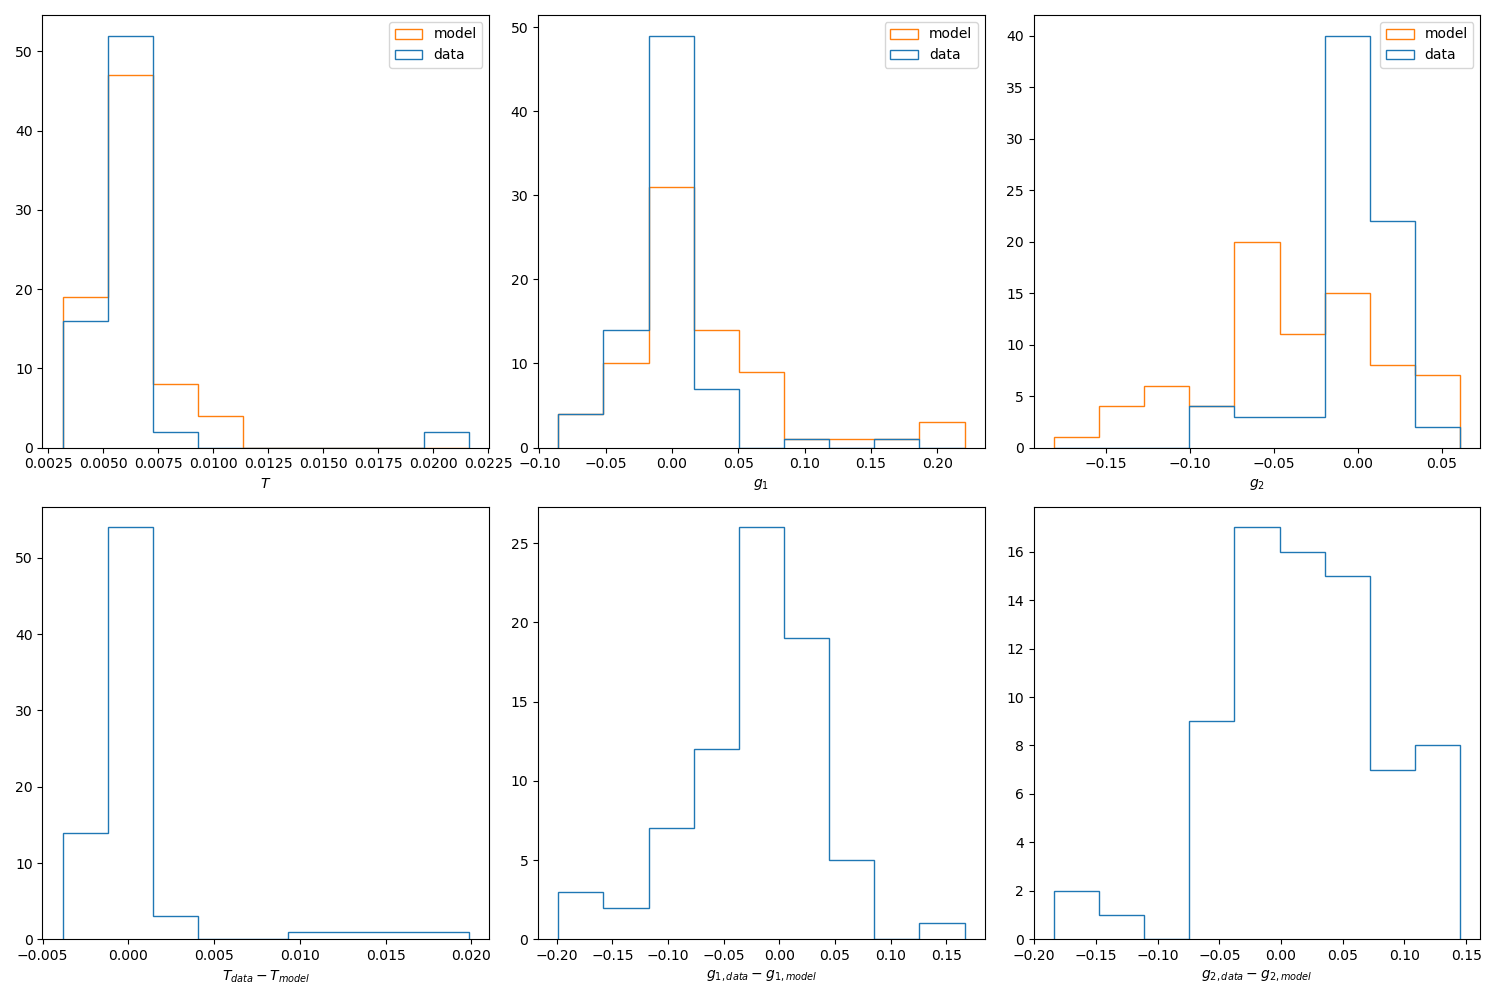
\includegraphics[width=.3\linewidth]{277.30/piff_shapes.png}\hfill
  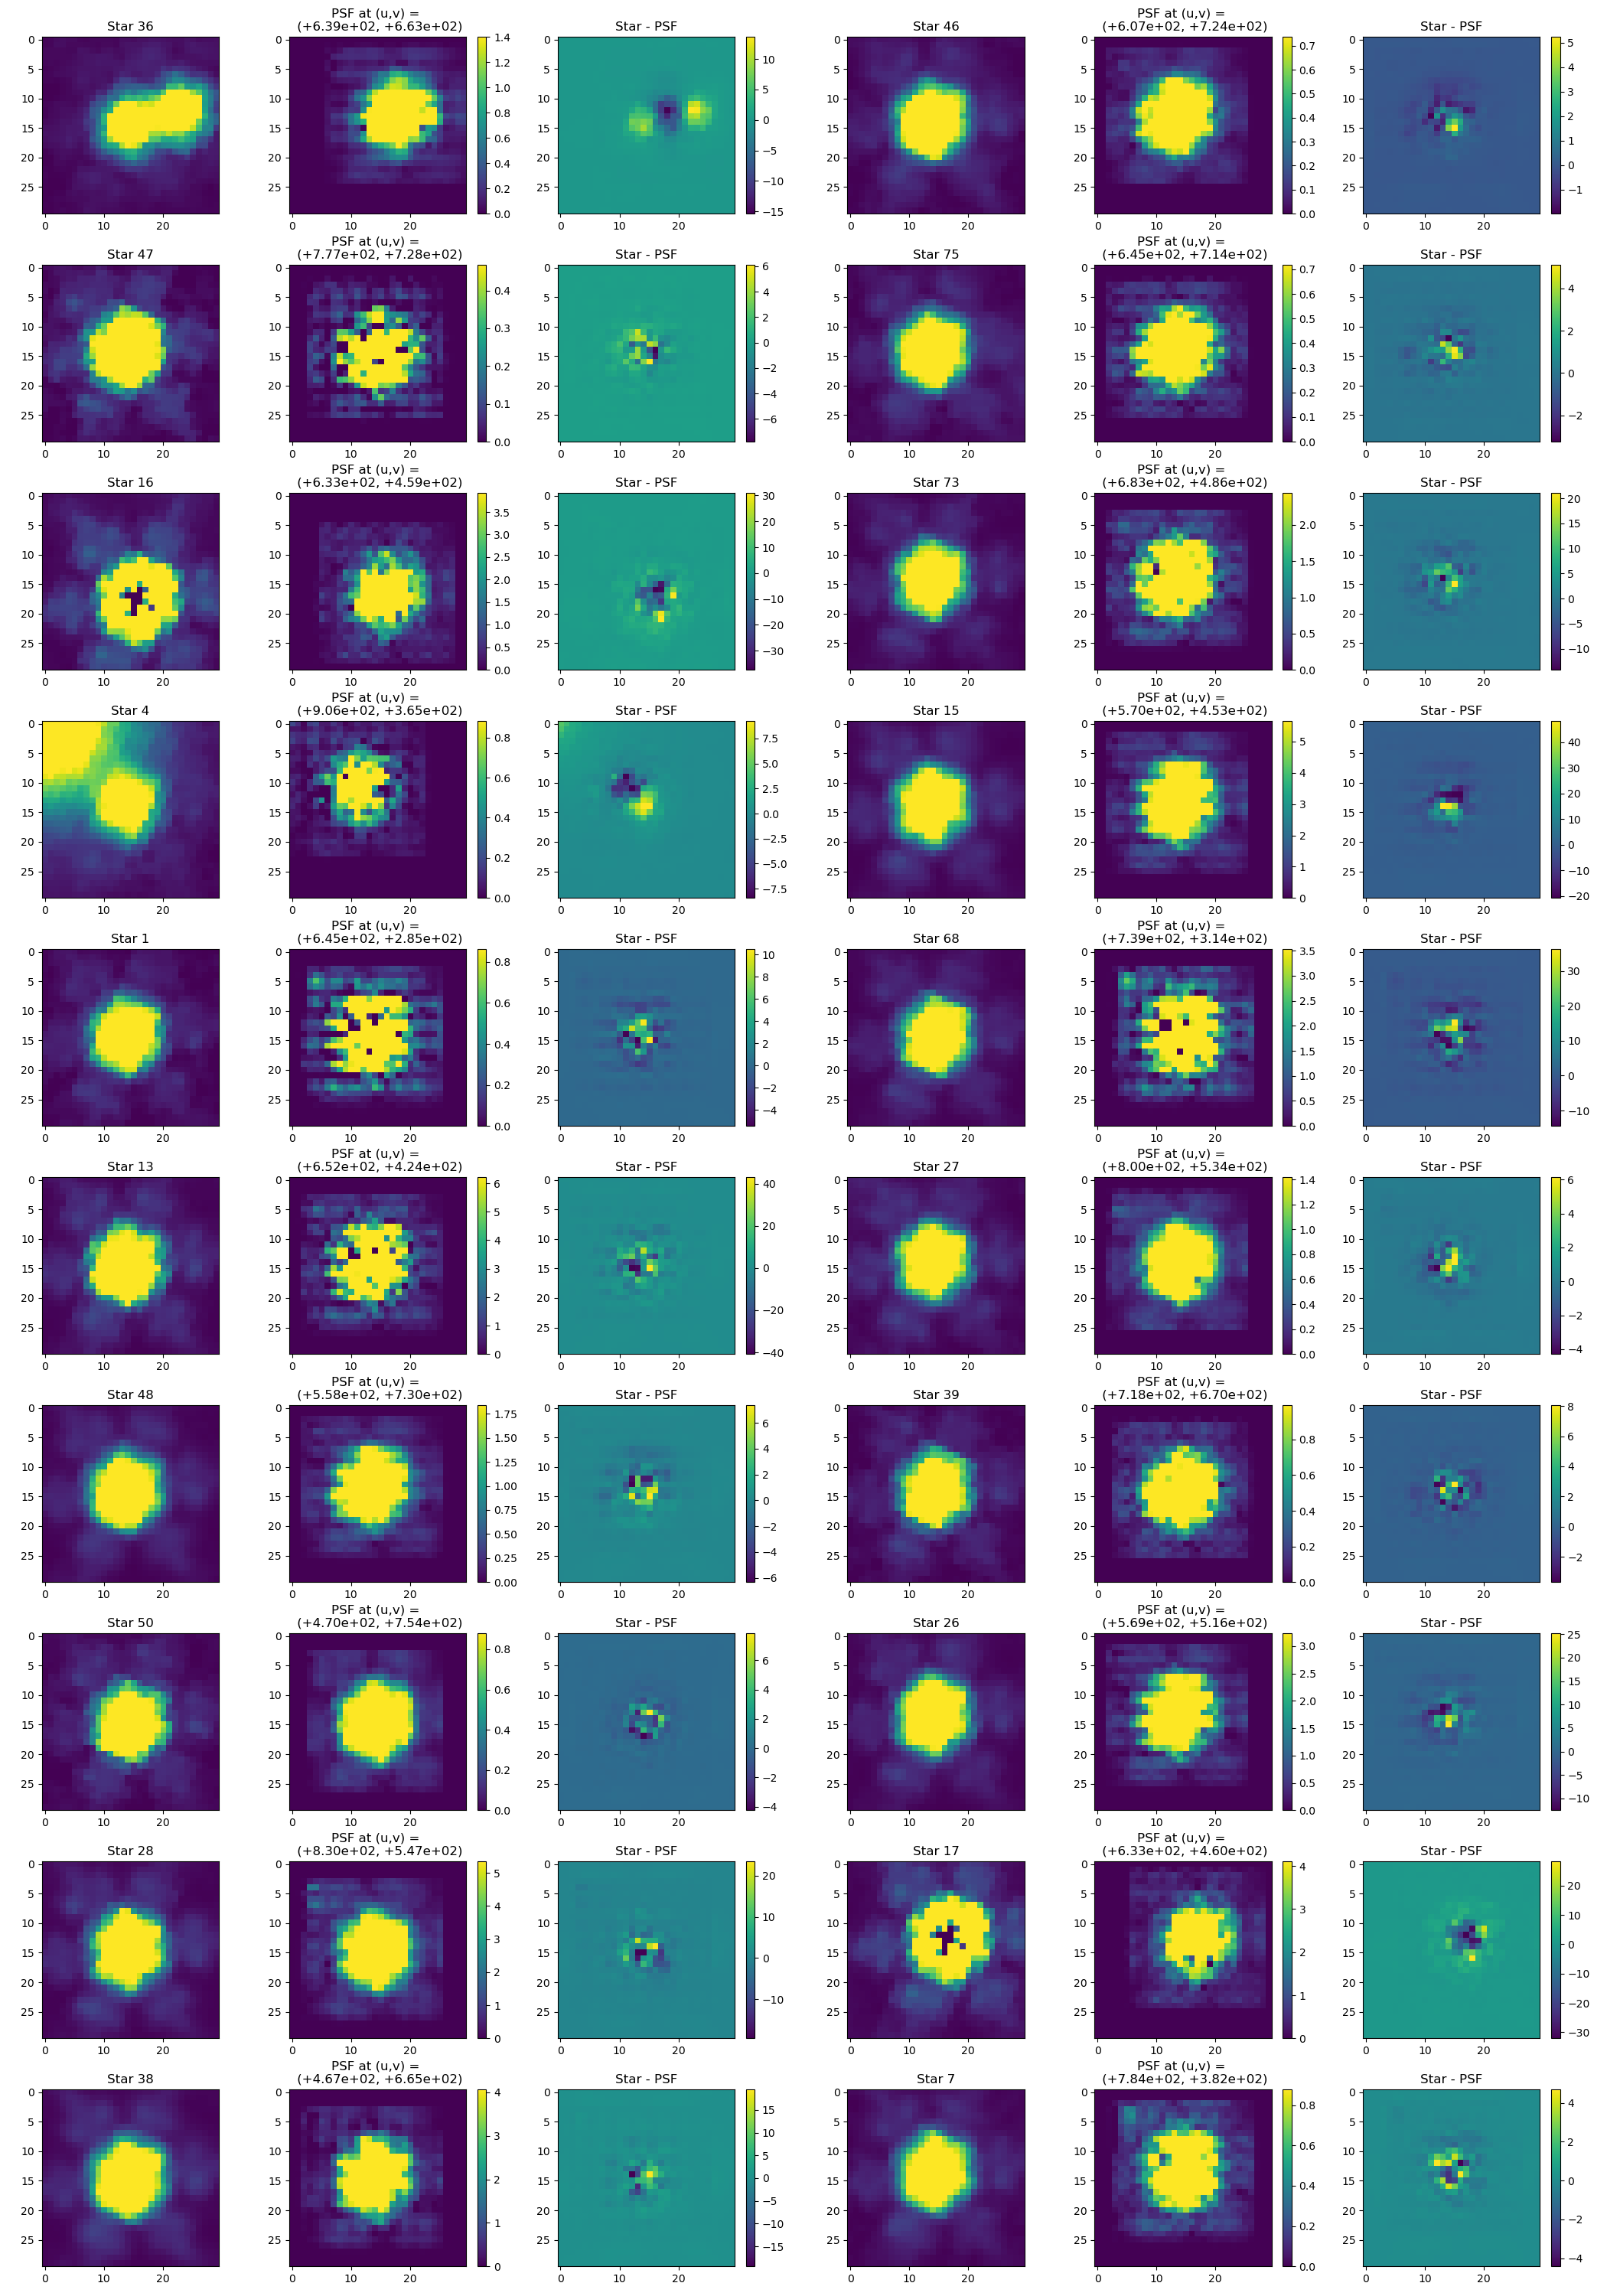
\includegraphics[width=.3\linewidth]{277.30/piff_stars.png}
  \end{subfigure}\par\medskip
  \begin{subfigure}{\linewidth}
  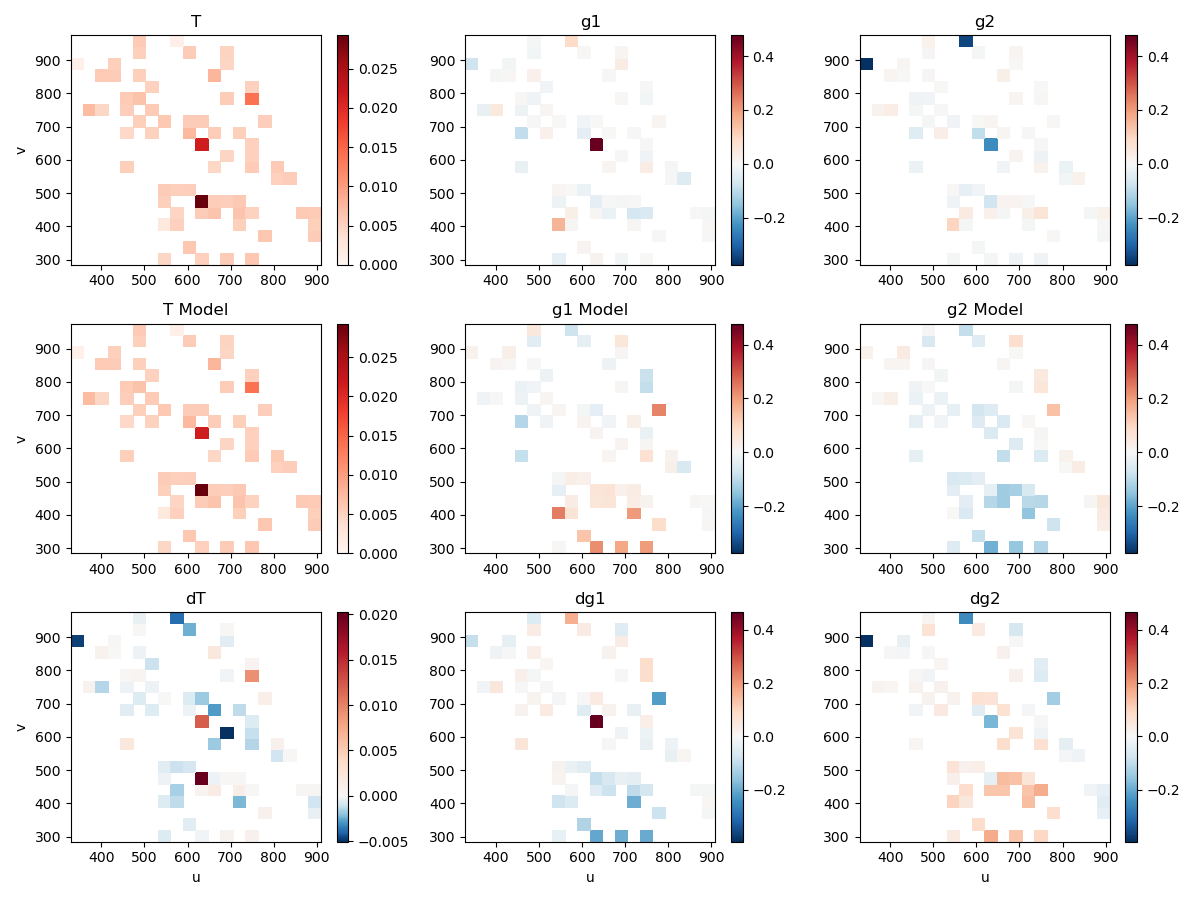
\includegraphics[width=.3\linewidth]{277.30/piff_twod.png}\hfill
  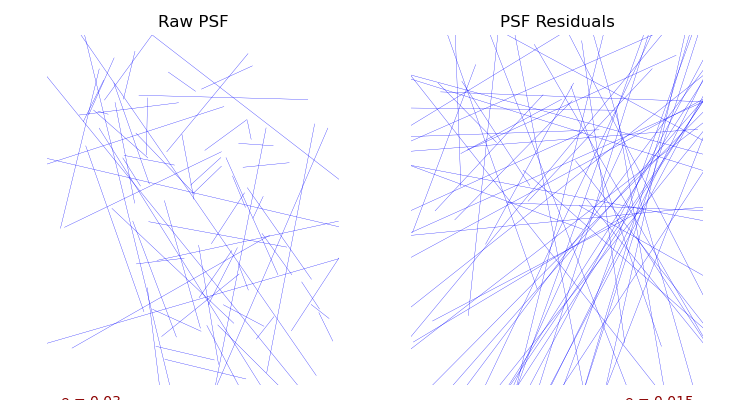
\includegraphics[width=.3\linewidth]{277.30/piff_whisker.png}\hfill
  \caption{f277w 30mas}
  \end{subfigure}\par\medskip


\end{figure}
\begin{figure}[!h]
  \begin{subfigure}{\linewidth}
  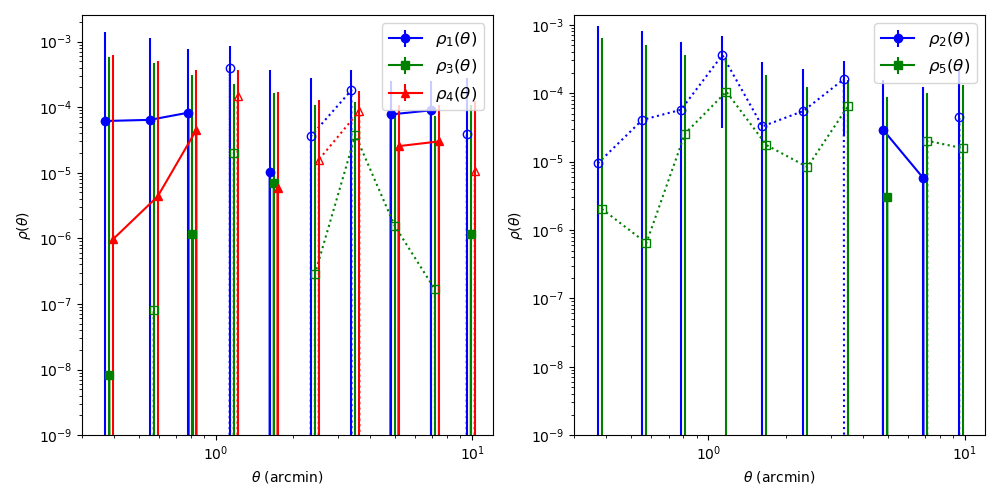
\includegraphics[width=.3\linewidth]{444.30/piff_rho.png}\hfill
  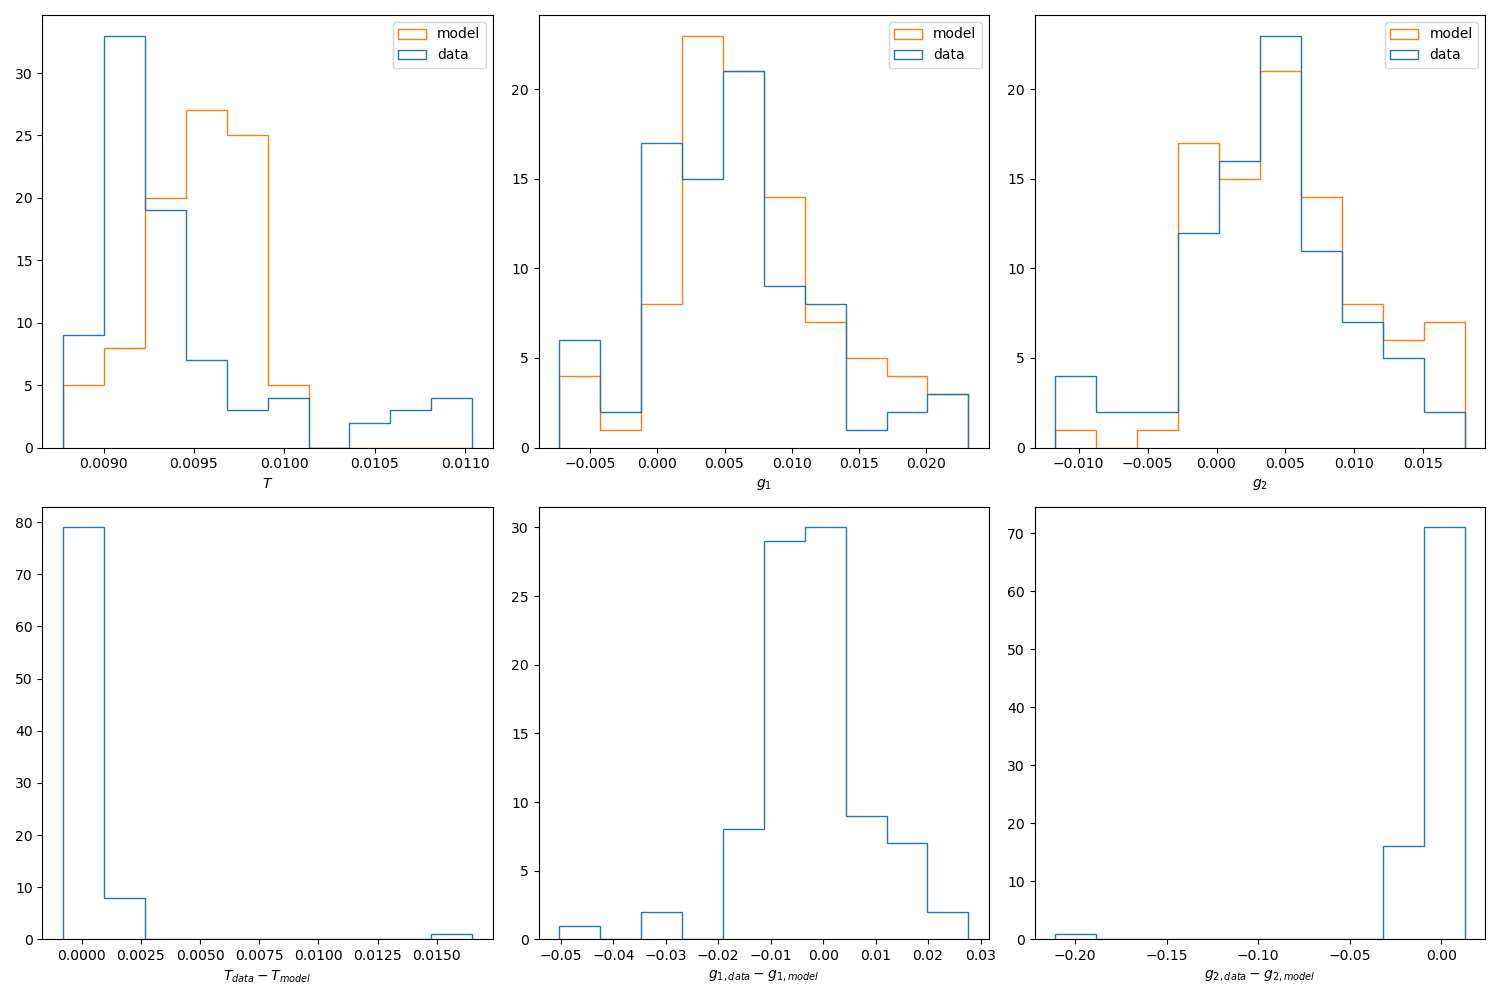
\includegraphics[width=.3\linewidth]{444.30/piff_shapes.png}\hfill
  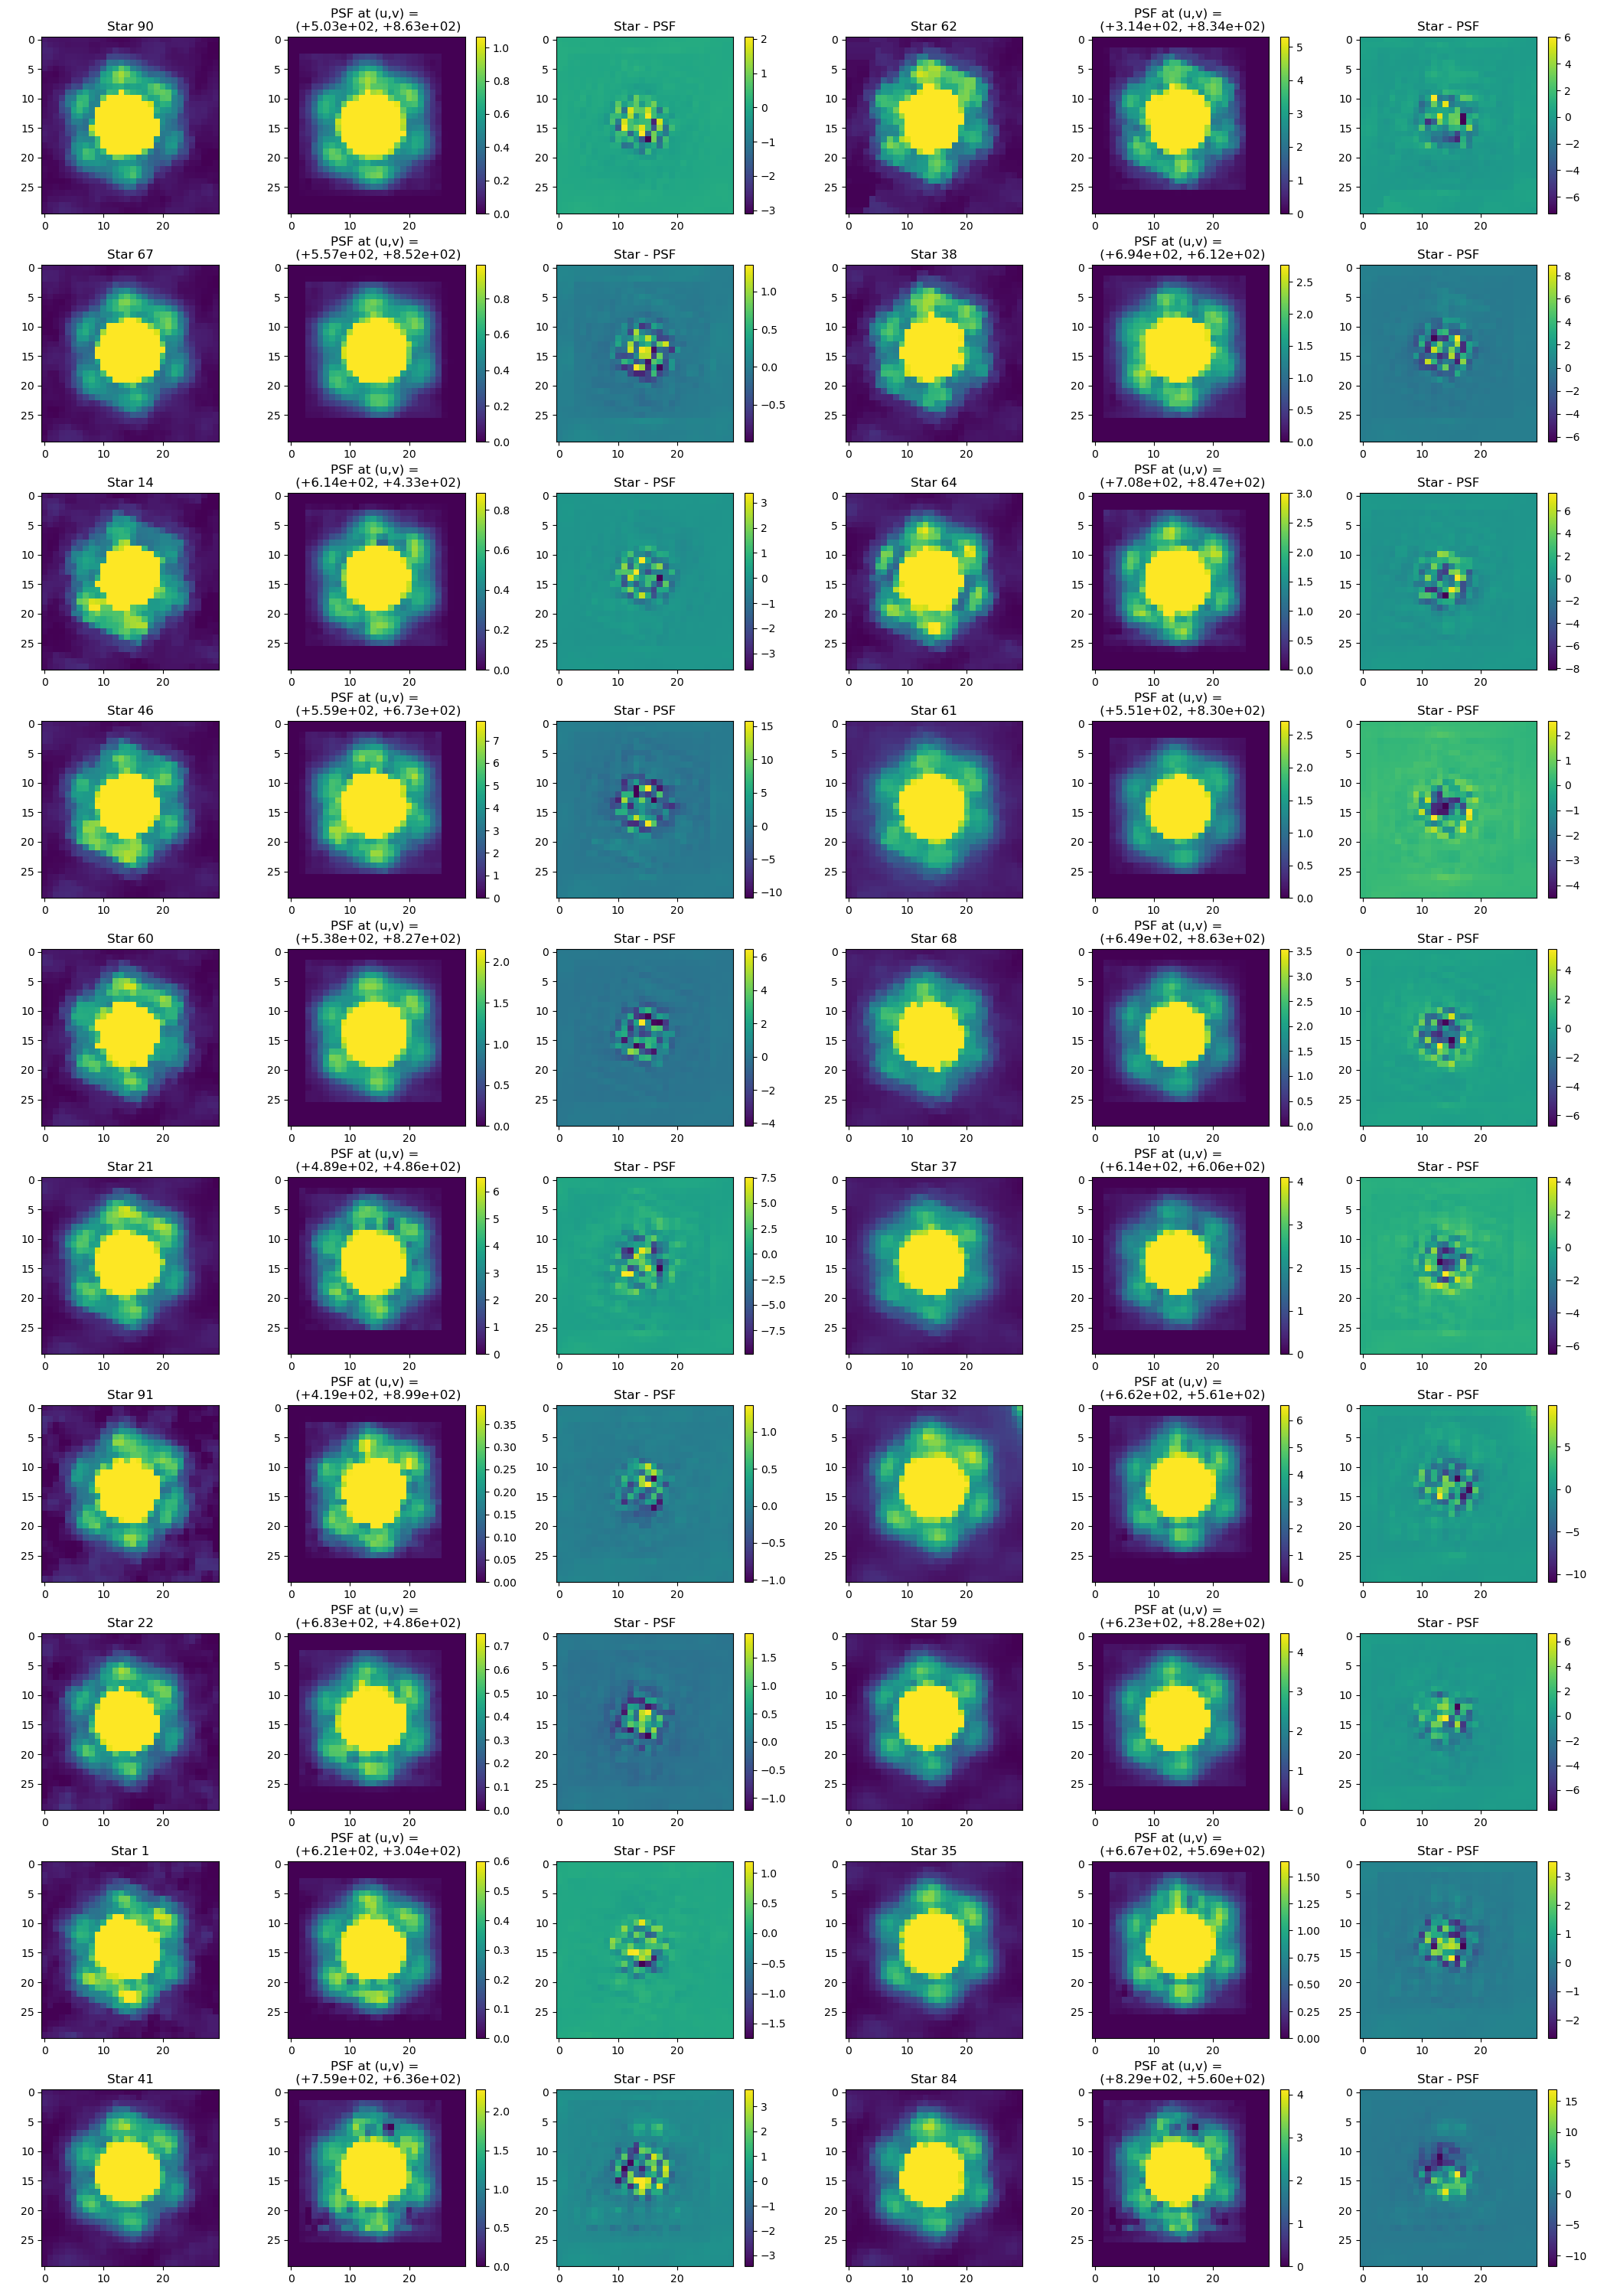
\includegraphics[width=.3\linewidth]{444.30/piff_stars.png}
  \end{subfigure}\par\medskip
  \begin{subfigure}{\linewidth}
  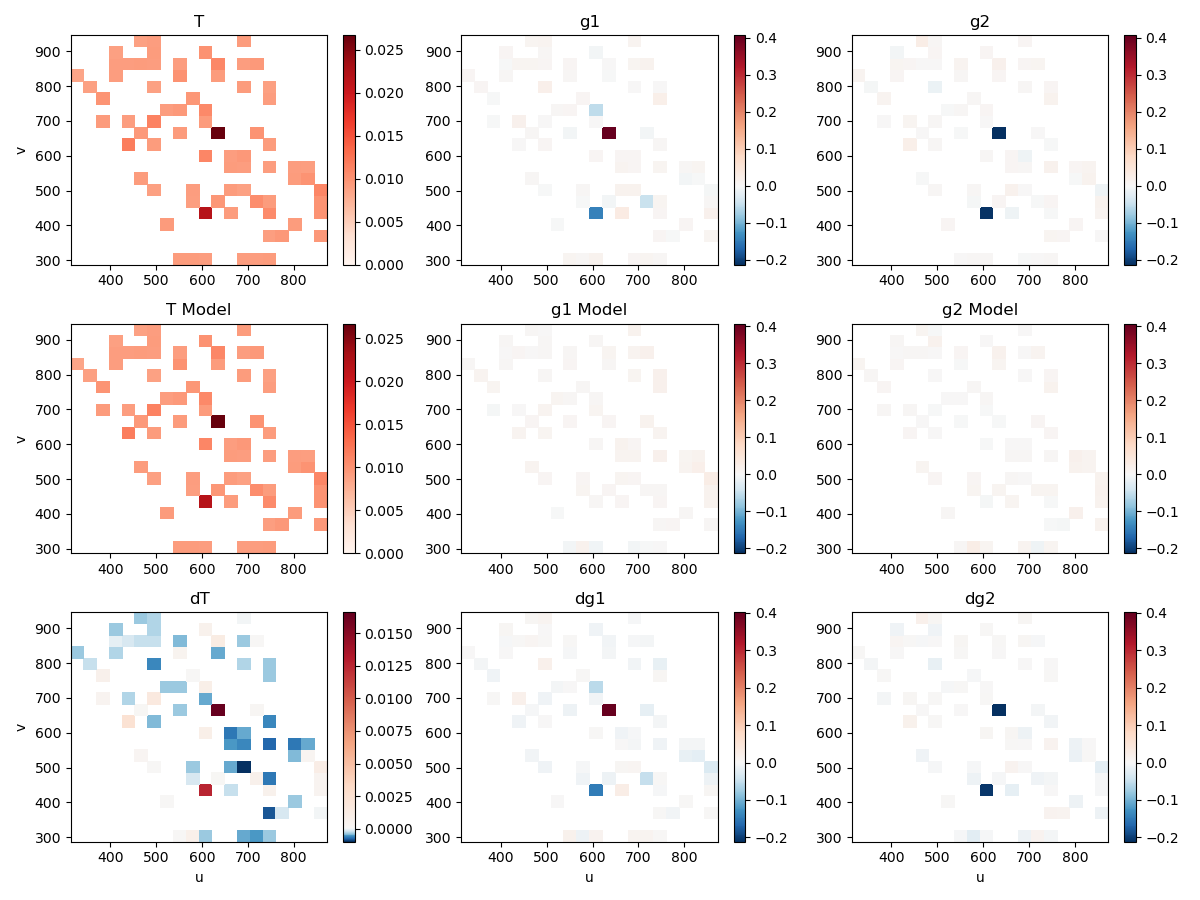
\includegraphics[width=.3\linewidth]{444.30/piff_twod.png}\hfill
  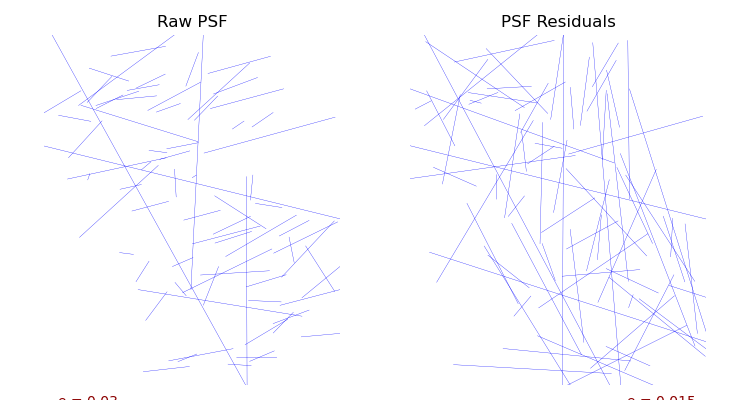
\includegraphics[width=.3\linewidth]{444.30/piff_whisker.png}\hfill
  \caption{f444w 30mas}
  \end{subfigure}\par\medskip


\end{figure}


\clearpage



\section{60 mas}
\begin{python}
# How large should the postage stamp cutouts of the stars be?
    stamp_size: 30

model:
    # This model uses a grid of pixels to model the surface brightness distribution.
    type: PixelGrid
    scale: 0.025      # NIRCam ative pixel scale
    size: 40          # Model is 24 x 24 in these pixels
\end{python}\\
?????
\\ \begin{figure}[!h]
  \begin{subfigure}{\linewidth}
  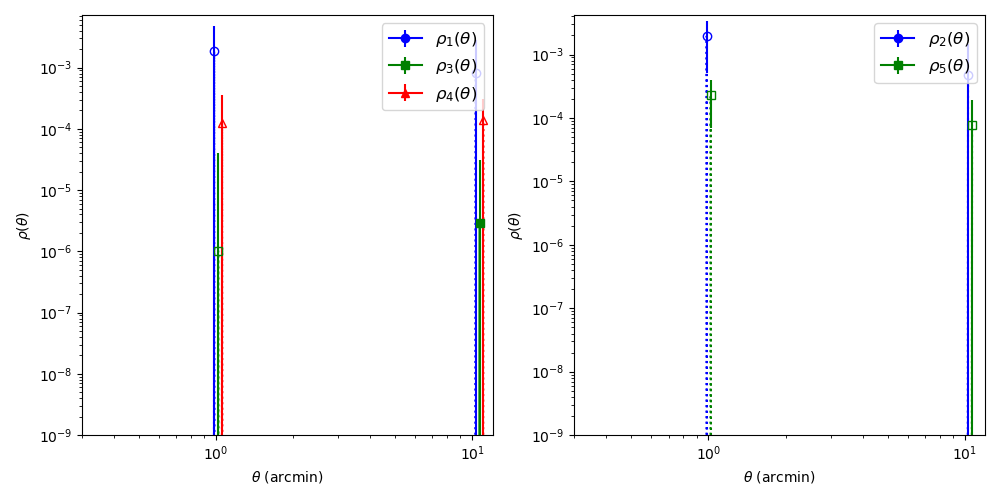
\includegraphics[width=.3\linewidth]{150.60/piff_rho.png}\hfill
  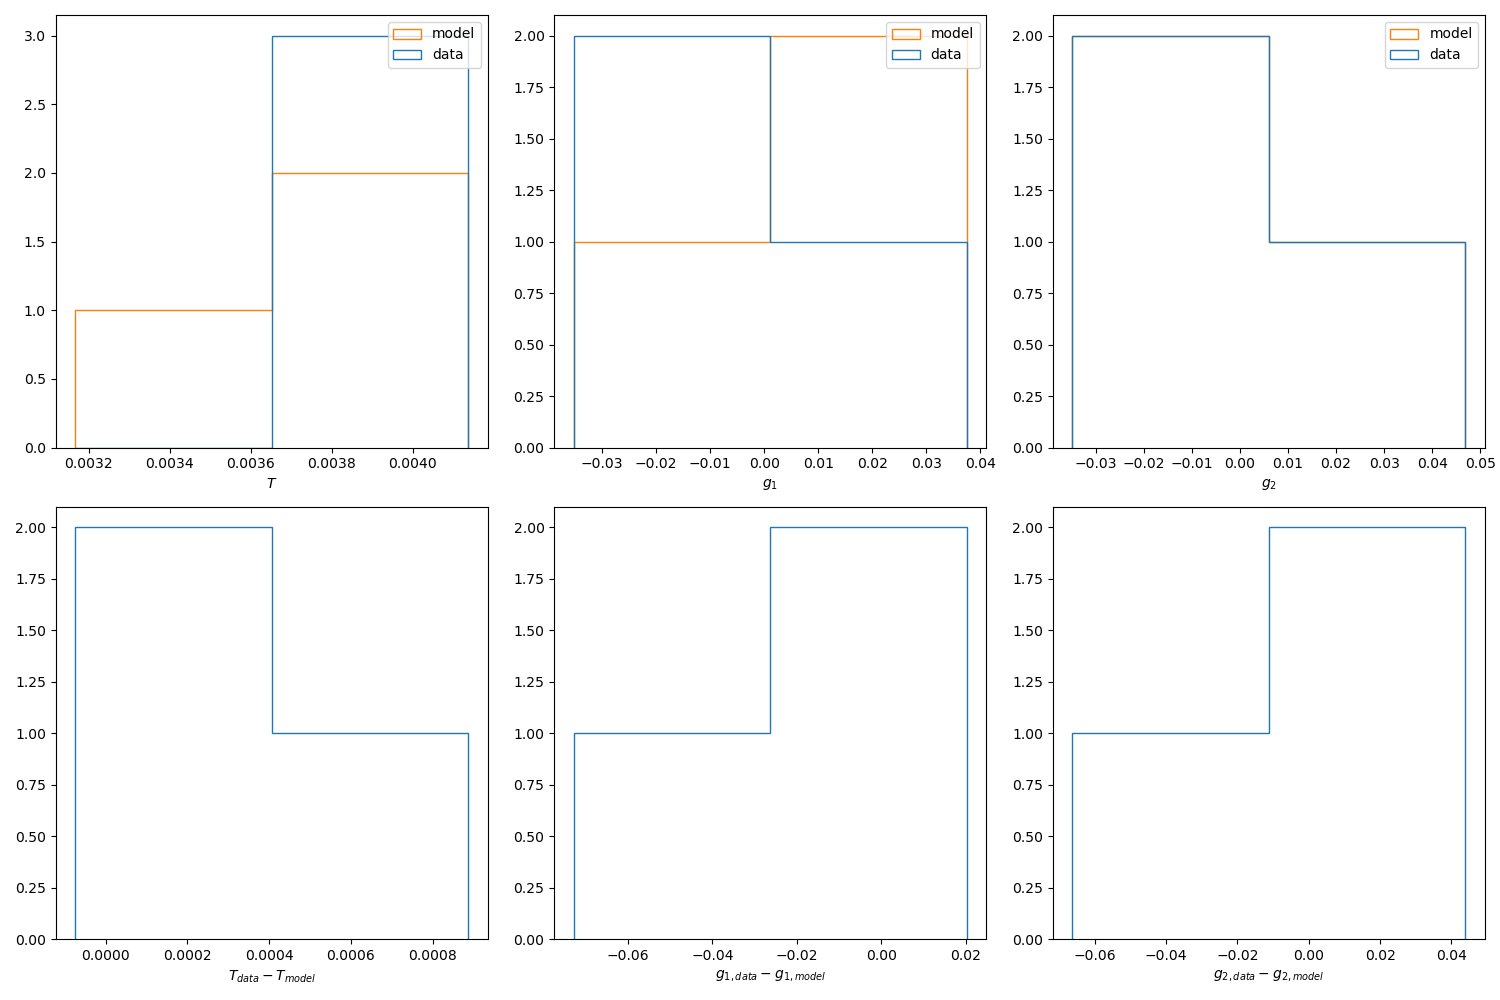
\includegraphics[width=.3\linewidth]{150.60/piff_shapes.png}\hfill
  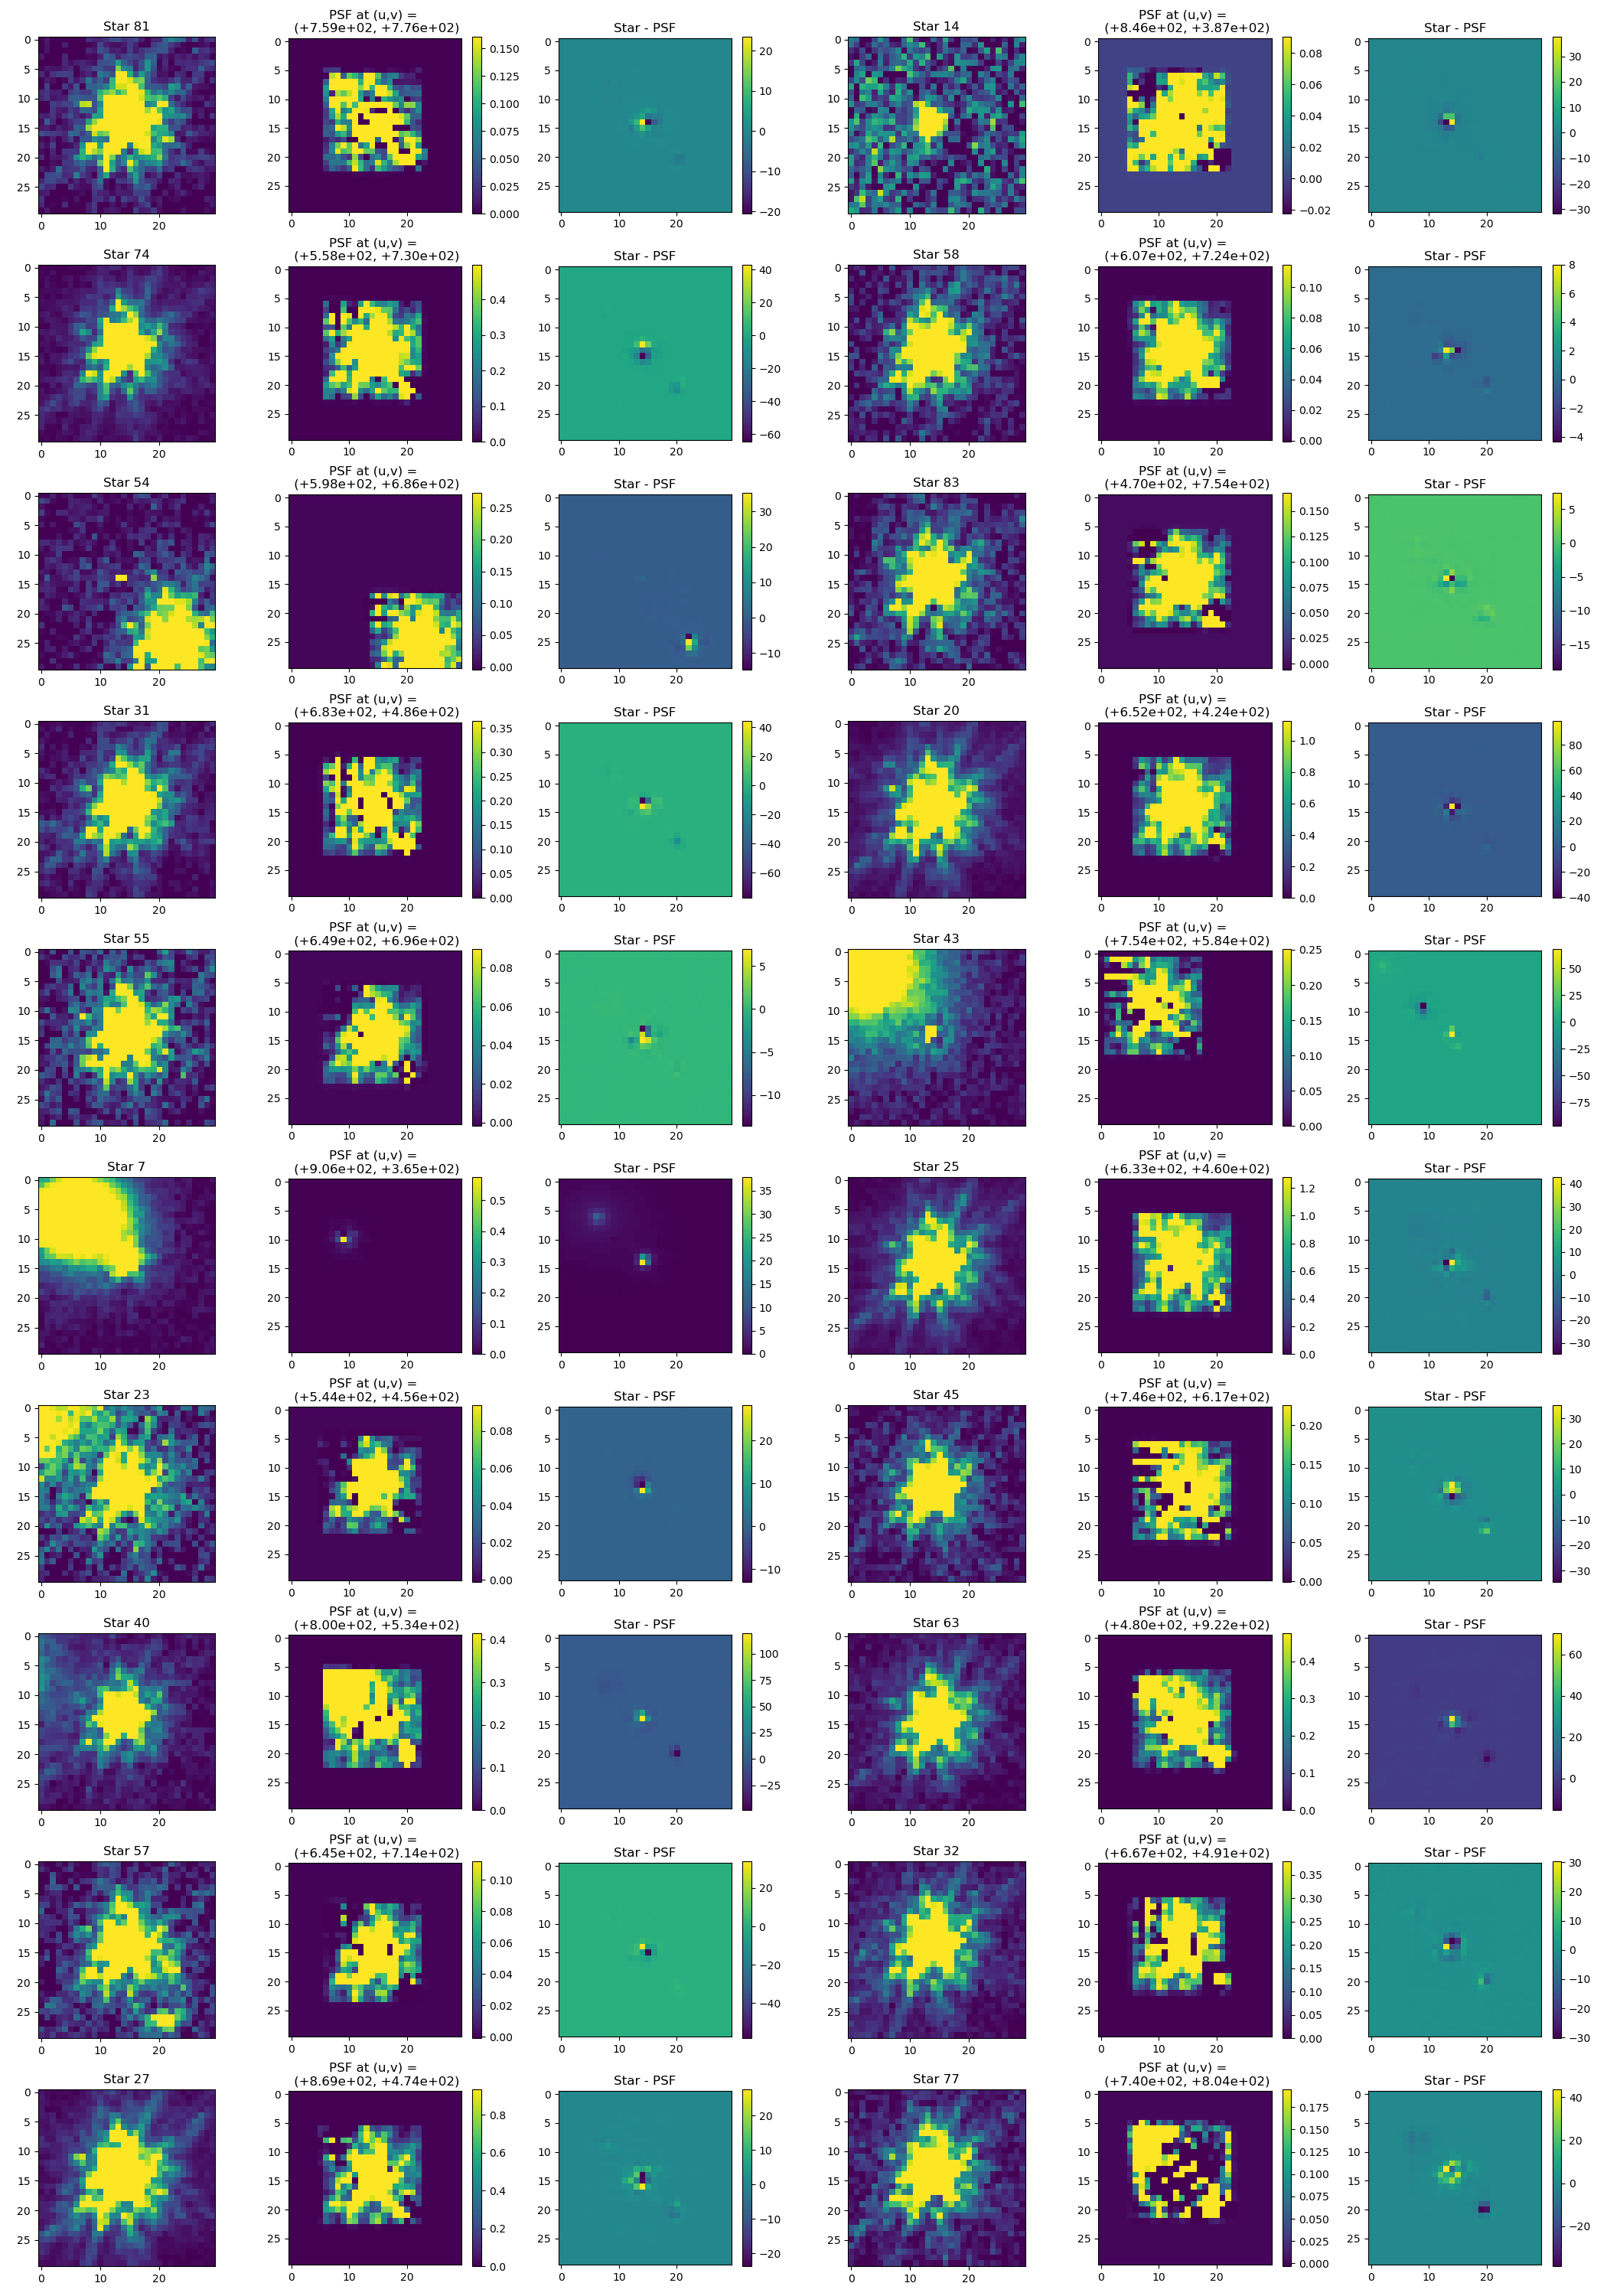
\includegraphics[width=.3\linewidth]{150.60/piff_stars.png}
  \end{subfigure}\par\medskip
  \begin{subfigure}{\linewidth}
  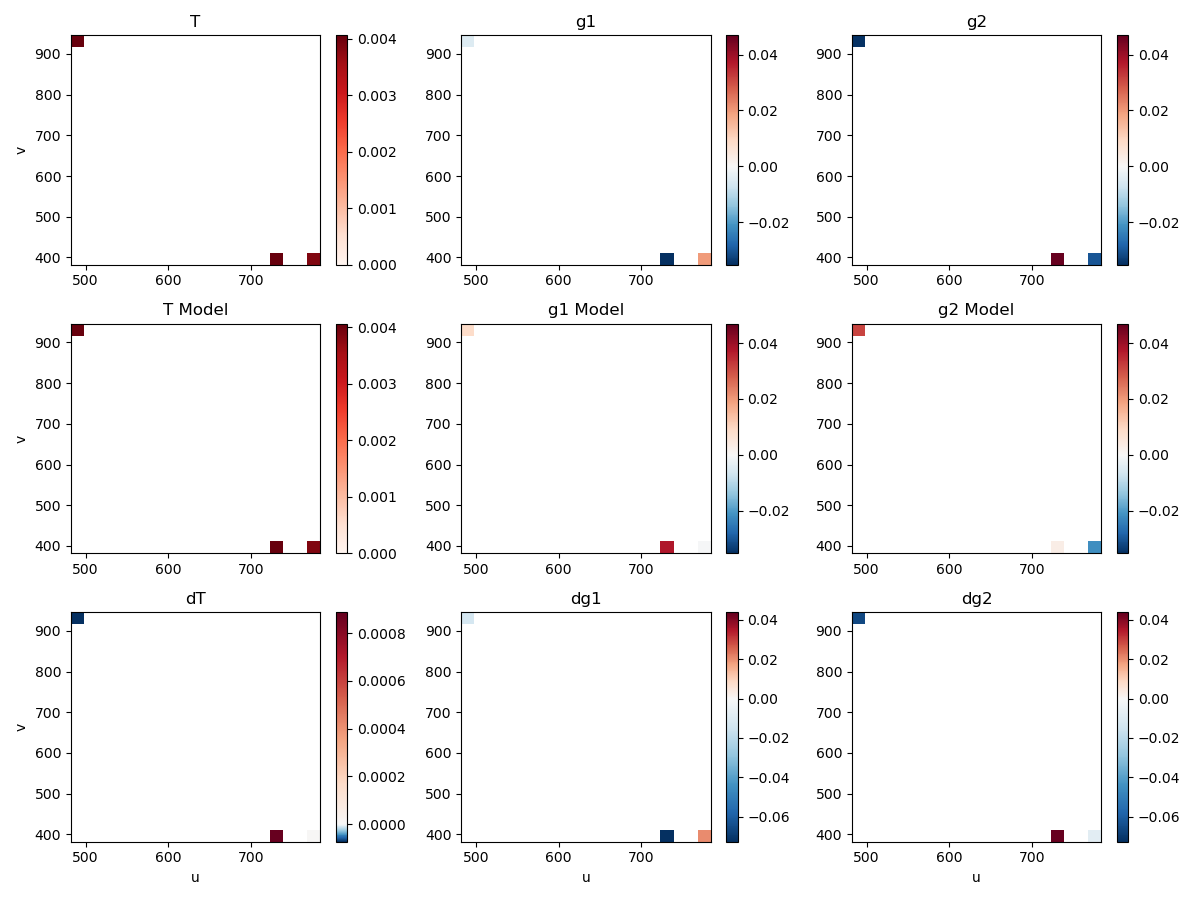
\includegraphics[width=.3\linewidth]{150.60/piff_twod.png}\hfill
  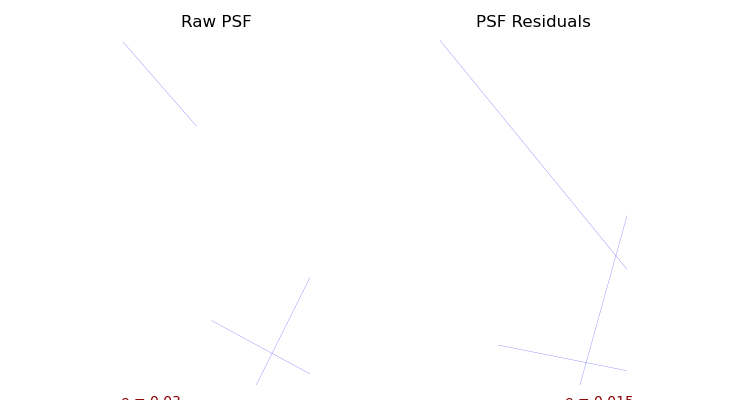
\includegraphics[width=.3\linewidth]{150.60/piff_whisker.png}\hfill
  \caption{f150w 30mas }
  \end{subfigure}\par\medskip


\end{figure}\\
\begin{python}
# How large should the postage stamp cutouts of the stars be?
    stamp_size: 30

model:
    # This model uses a grid of pixels to model the surface brightness distribution.
    type: PixelGrid
    scale: 0.025      # NIRCam ative pixel scale
    size: 36          # Model is 24 x 24 in these pixels
\end{python}\\
\underline{\textbf{NB:}} This worked really well on simulated data for f444w 60mas. Not working on F150w 60mas. \clearpage
\begin{python}
# How large should the postage stamp cutouts of the stars be?
    stamp_size: 30

model:
    # This model uses a grid of pixels to model the surface brightness distribution.
    type: PixelGrid
    scale: 0.025      # NIRCam ative pixel scale
    size: 54          # Model is 24 x 24 in these pixels
\end{python}\\
\begin{figure}[!h]
  \begin{subfigure}{\linewidth}
  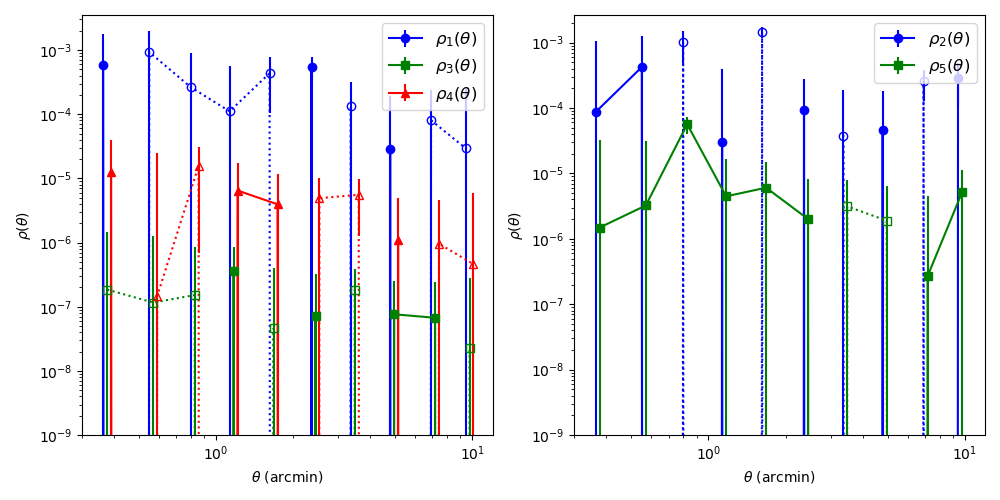
\includegraphics[width=.3\linewidth]{444.60.54/piff_rho.png}\hfill
  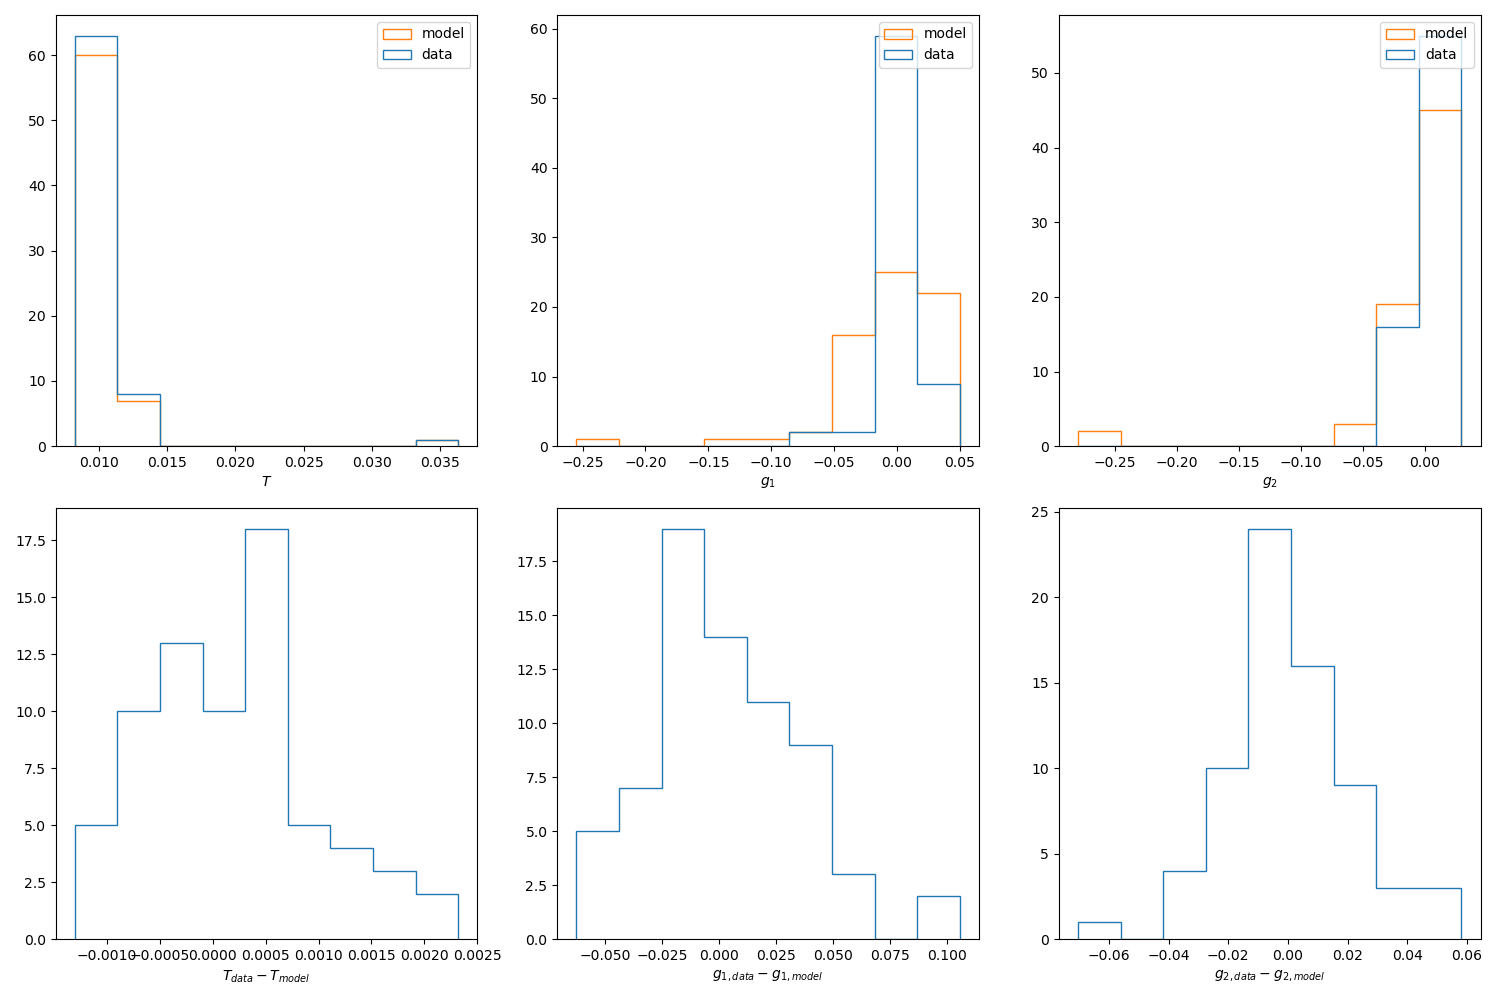
\includegraphics[width=.3\linewidth]{444.60.54/piff_shapes.png}\hfill
  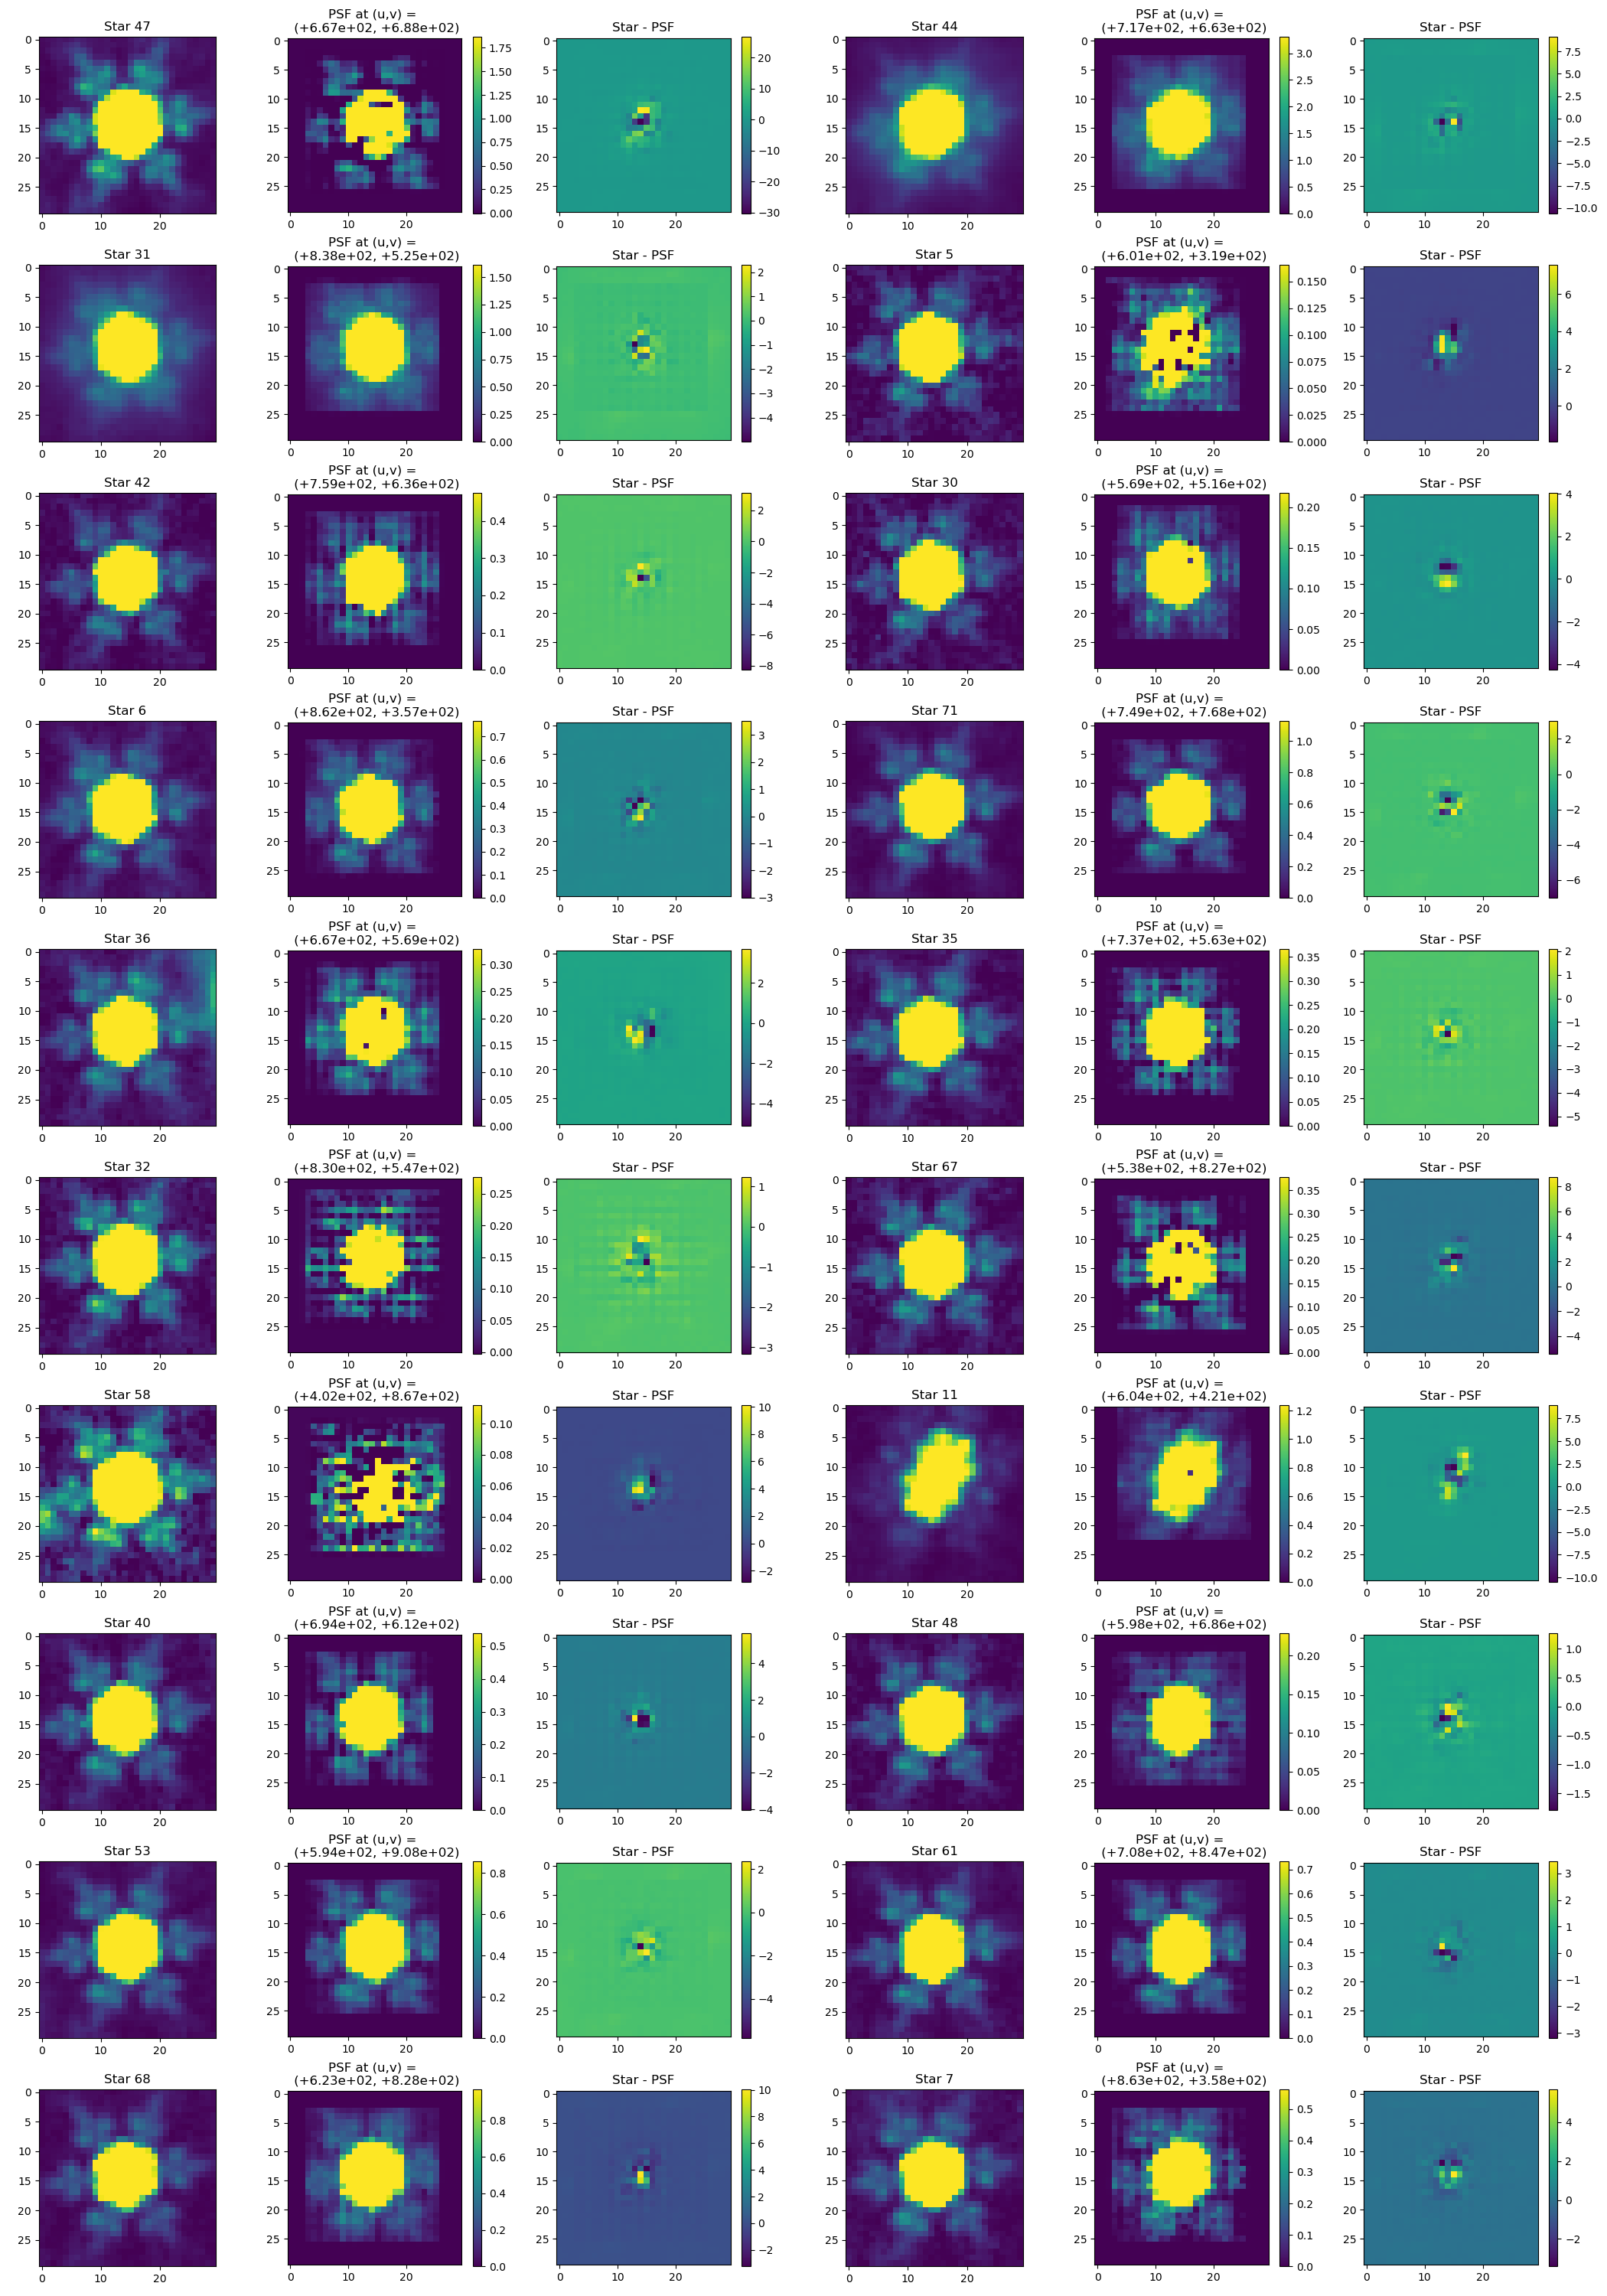
\includegraphics[width=.3\linewidth]{444.60.54/piff_stars.png}
  \end{subfigure}\par\medskip
  \begin{subfigure}{\linewidth}
  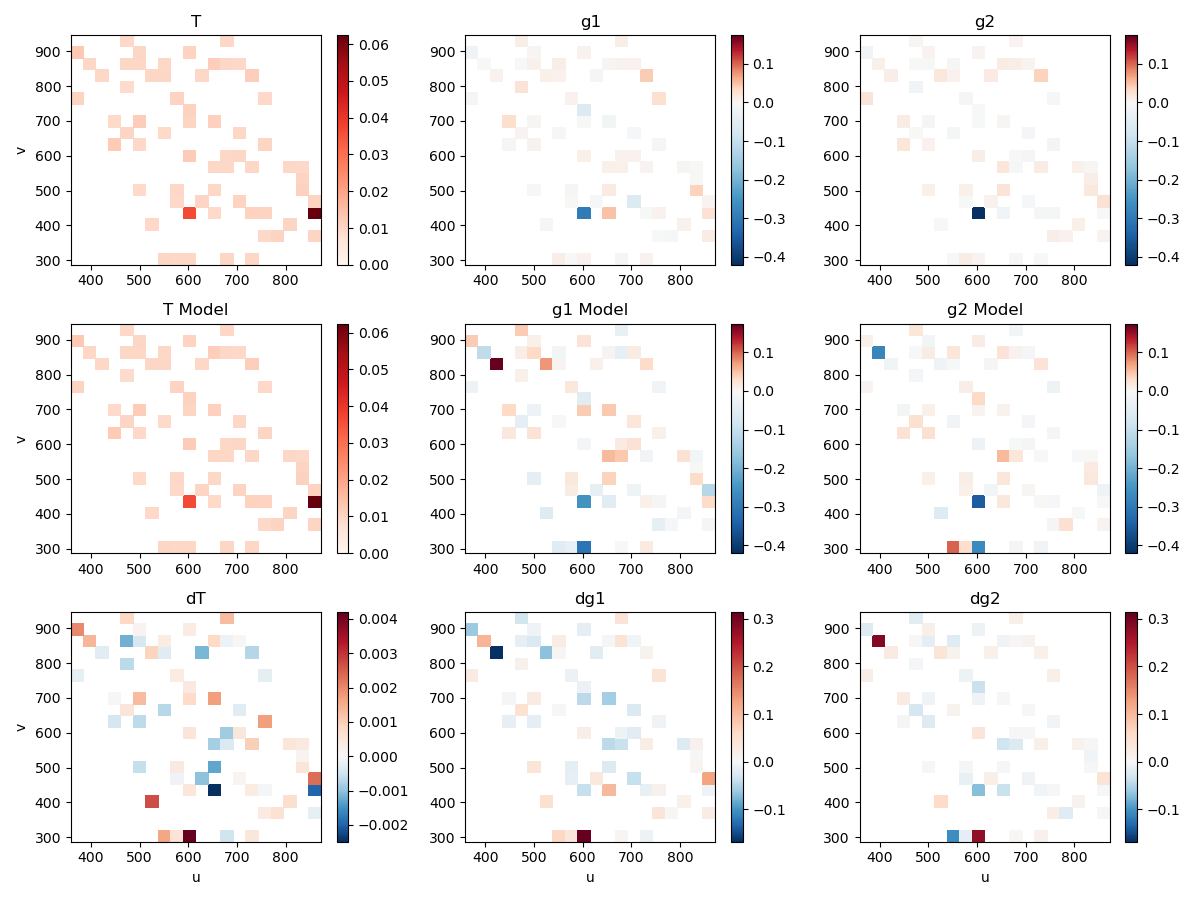
\includegraphics[width=.3\linewidth]{444.60.54/piff_twod.png}\hfill
  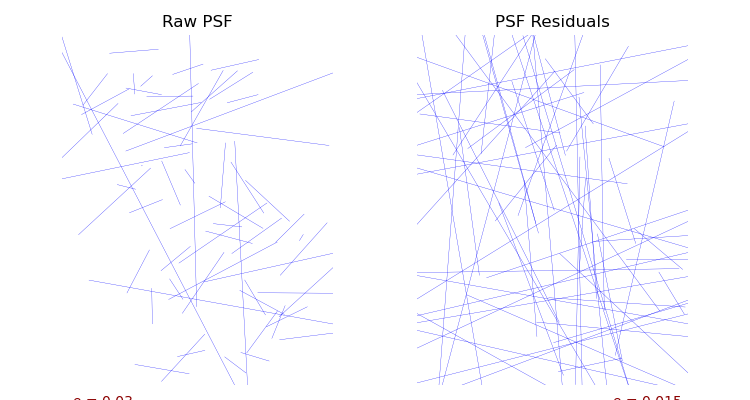
\includegraphics[width=.3\linewidth]{444.60.54/piff_whisker.png}\hfill
  \caption{f444w 60mas}
  \end{subfigure}\par\medskip


\end{figure}\\

\begin{figure}[!h]
  \begin{subfigure}{\linewidth}
  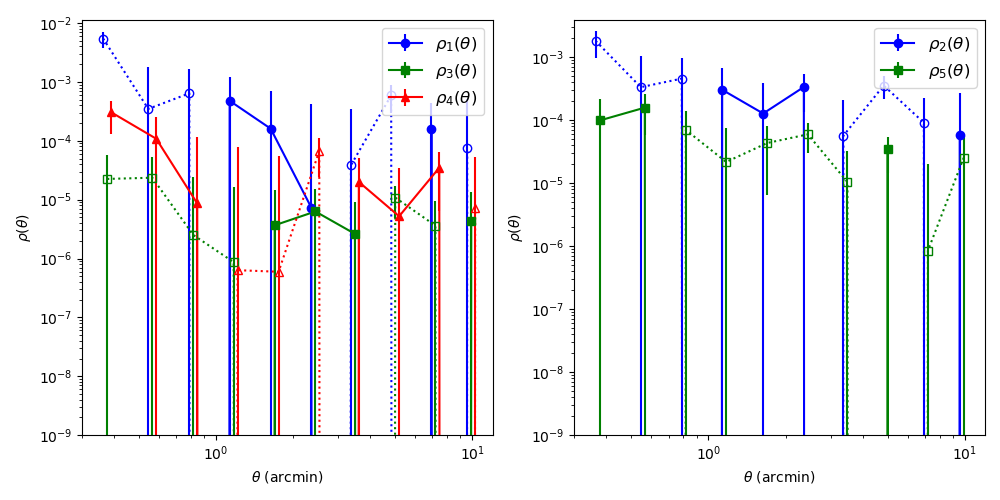
\includegraphics[width=.3\linewidth]{277.60.54/piff_rho.png}\hfill
  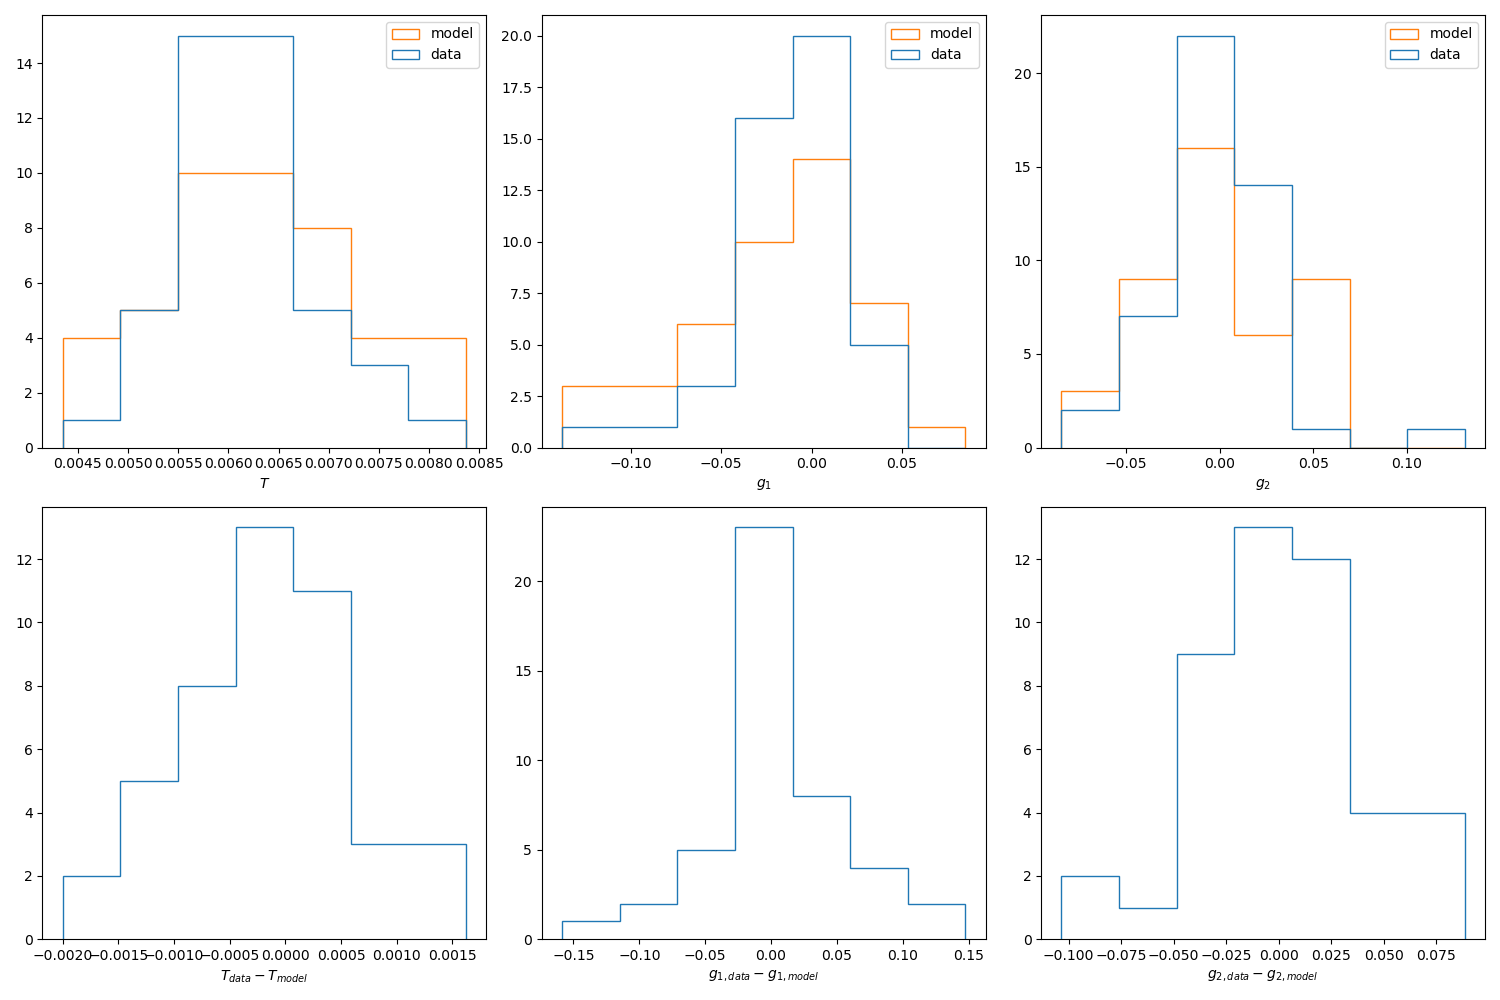
\includegraphics[width=.3\linewidth]{277.60.54/piff_shapes.png}\hfill
  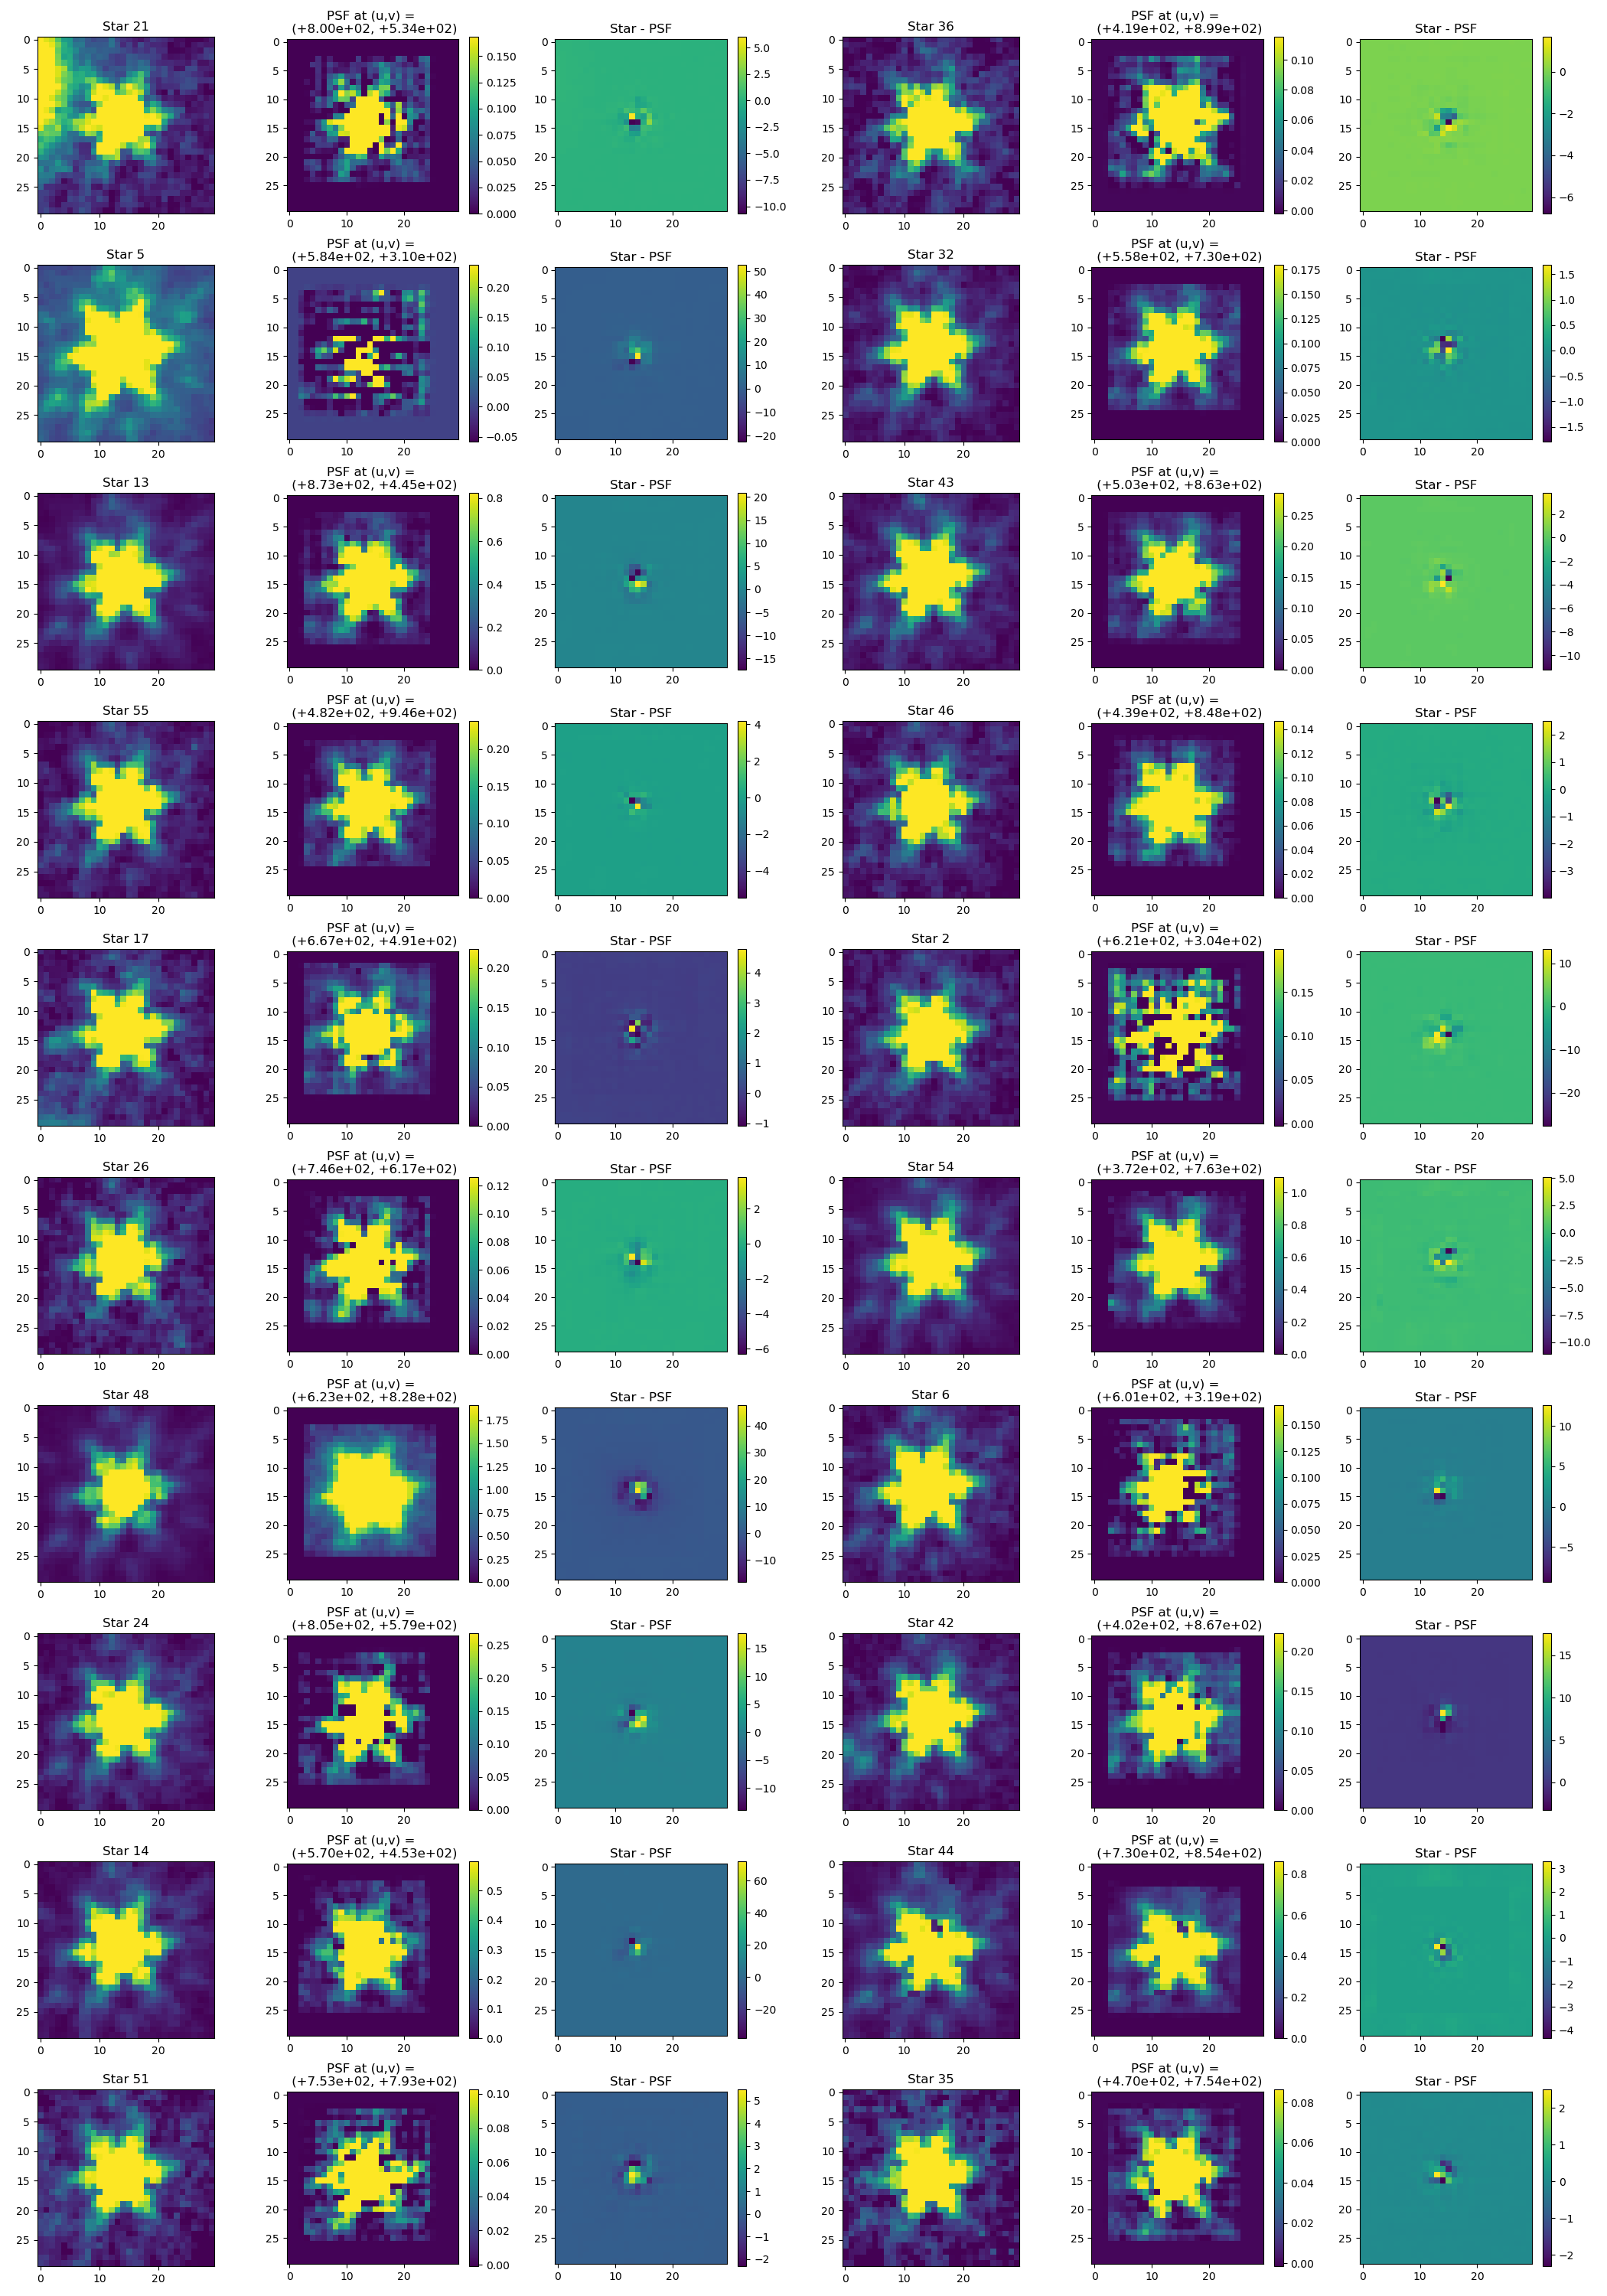
\includegraphics[width=.3\linewidth]{277.60.54/piff_stars.png}
  \end{subfigure}\par\medskip
  \begin{subfigure}{\linewidth}
  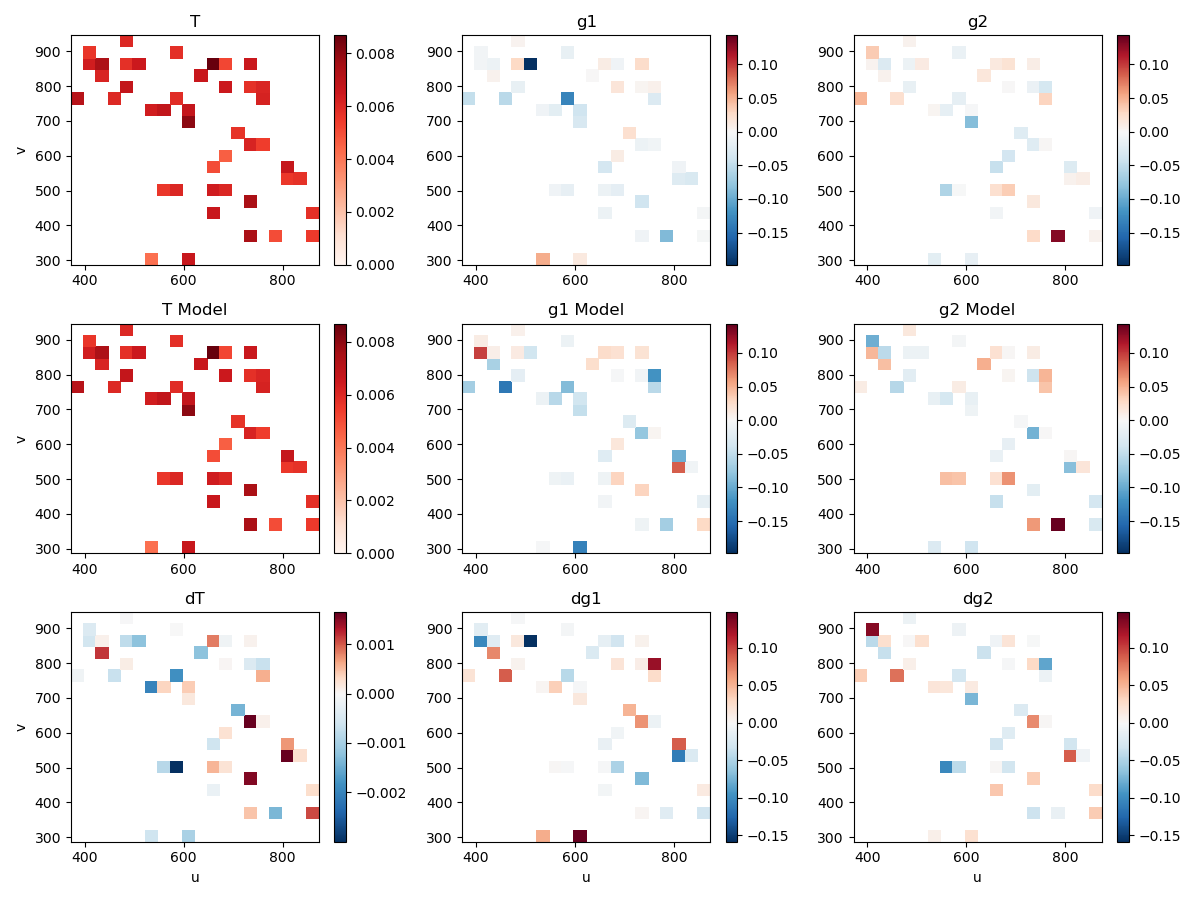
\includegraphics[width=.3\linewidth]{277.60.54/piff_twod.png}\hfill
  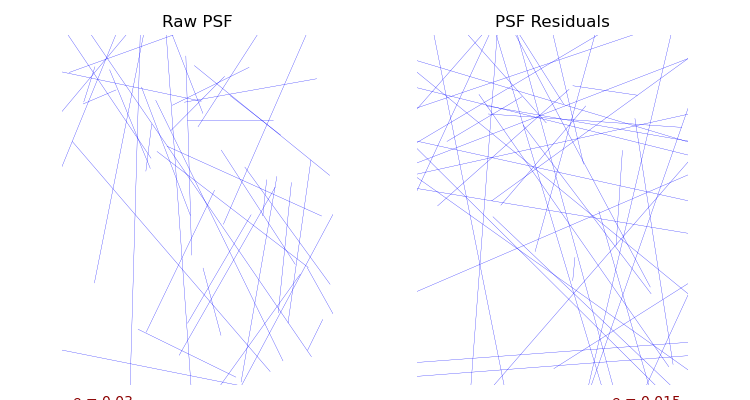
\includegraphics[width=.3\linewidth]{277.60.54/piff_whisker.png}\hfill
  \caption{f277w 60mas}
  \end{subfigure}\par\medskip


\end{figure}\\





\clearpage
\noindent {\fbox{\it Still to Do / Notes}}\\ 
\begin{itemize}
    \item Attended talk Blazek shared
    \item Why does iteration number vary?
    \item Seem to be rejecting a lot of stars...
    \item I think I am ready to start creating my own metrics
    \item Fabian 
    \item SUMS
\end{itemize}

















\end{document}
%%------------ Arman Shokrollahi--------------%%
